\documentclass[spanish,final]{thesis} [2015/30/06 v1.0]

\author{T�cn. Carlos Brayan R�mila Chorens}
\title{Aplicaci�n Web para la Mejora en la Gesti�n de Servicios de Transconsul S.A.}
\ucicenter{}
\facultynum{4}
\addtutor[Tutora]{MSc. Yadira Ram�rez Rodr�guez}

\thought{La eficaz gesti�n de citas y servicios legales no solo es una necesidad operativa, sino un pilar fundamental para garantizar la confianza y satisfacci�n de nuestros clientes en cada interacci�n.  \\
 John Smith, Experto en Gesti�n Legal}
 
\dedicatory{A mi familia, amigos, compa�eros y profesores, quienes con su amor, apoyo, sabidur�a y aliento han sido mi mayor inspiraci�n y motivaci�n en cada paso del camino. Este trabajo est� dedicado a ustedes, quienes han hecho posible este logro con su constante presencia y ayuda incondicional.}

\acknowledgment{Quiero expresar mi m�s profundo agradecimiento a todas las personas que han sido parte de este viaje acad�mico. A mi familia, por su amor incondicional y su constante apoyo en cada desaf�o que he enfrentado. A mis amigos, por estar siempre presentes, brind�ndome su amistad y aliento en los momentos dif�ciles. A mis compa�eros, por compartir este camino conmigo, por los momentos de colaboraci�n y aprendizaje mutuo. Y a mis profesores, por su orientaci�n, sabidur�a y dedicaci�n, que han sido fundamentales para mi crecimiento acad�mico y personal. \\
En especial, quiero agradecer a mi tutora y profesora, M.Sc. Yadira Ram�rez Rodr�guez, por su invaluable gu�a y apoyo durante todo el proceso de investigaci�n y redacci�n de esta tesis. Su paciencia, experiencia y compromiso han sido fundamentales para alcanzar este logro. \\
Por �ltimo, pero no menos importante, quiero agradecerme a m� mismo por mi perseverancia, determinaci�n y dedicaci�n para alcanzar mis metas. Sin mi propia fuerza interior y convicci�n, este logro no habr�a sido posible.}

\abstract{Lorem mioipsum dolor sit amet, consectetuer adipiscing elit. Ut purus elit, vestibulum ut, placerat ac, adipiscing vitae, felis. Curabitur dictum gravida mauris. Nam arcu libero, nonummy eget, consectetuer id, vulputate a, magna.}

\keywords{word1, word2, word3}

\newglossaryentry{Engine}{name=engine, description={part of a program which handles certain types of data (Computers)}}
\newacronym{UCI}{UCI}{Universidad de las Ciencias Inform�ticas}
\newacronym{S.A.}{S.A.}{Sociedad An�nima}
\newacronym{XP}{XP}{Progrmaci�n Extrema}
\newacronym{RSS}{RSS}{Sindicaci�n Realmente Simple} % por sus siglas en ingl�s (Really Simple Syndication )
\newacronymeng{SCADA}{SCADA}{Supervisi�n, Control y Adquisici�n de Datos}
\newacronym{SQL}{SQL}{Lenguaje de Consulta Estructurada} % por sus siglas en ingl�s (Structured Query Language)
\newacronym{CRC}{CRC}{Class Responsibility Collaboration} % por sus siglas en ingl�s (Structured Query Language)
\newacronym{GoF}{GoF}{Gang of Four} % por sus siglas en ingl�s (Structured Query Language)
\newacronym{GRASP}{GRASP}{General Responsibility Assignment Software Patterns}


\addbibresource{carlosbrc.bib}

\begin{document}
  \maketitle
  
  \introduction

El desarrollo vertiginoso de las nuevas tecnolog�as, particularmente en las ramas de la inform�tica y las
telecomunicaciones, evidencia que es esta la era con mayor evoluci�n cient�fico-t�cnica de todos los
tiempos. Este desarrollo tecnol�gico acelerado incide sustancialmente en el mundo referencial del ser
humano, pues, si bien facilita la adquisici�n y almacenamiento de nuevos conocimientos, nuevos enfoques
y/o perspectivas y acciones que ayer mismo parec�an inaccesibles pero, de la misma manera, le est�n
condicionando y obligando a adaptaciones y replanteamientos en todos los �rdenes de su existencia. \\

En el campo del desarrollo de software tambi�n se constata un avance sin precedentes a nivel mundial, lo
cual posibilita la construcci�n de aplicaciones y sistemas inform�ticos capaces de solventar la amplia
amalgama de problemas te�ricos y pr�cticos de la sociedad. Diversas �reas de la vida diaria se ven
afectadas continuamente por la industria del software, tales como los aeropuertos, los bancos, las grandes
empresas, las instituciones policiales y militares entre otras. \\

Los sistemas de gesti�n son una rama importante dentro de la industria del desarrollo de software puesto
que resuelven un gran n�mero de situaciones a trav�s de la automatizaci�n de procesos, lo cual facilita el
trabajo en oficinas, elimina el tiempo de respuesta por parte de los proveedores de servicios a la
poblaci�n, suprime engorrosos bloques de papeles, propicia el trabajo de los seres humanos con grandes
vol�menes de informaci�n, el control y manipulaci�n de estad�sticas y una innumerable cantidad de
beneficios y posibilidades m�s, que a la postre, repercuten de forma positiva en la econom�a y la calidad
de vida de todos aquellos pa�ses que explotan este tipo de sistemas inform�ticos. \\

En Cuba, con la intenci�n de utilizar la amplia gama de posibilidades que brinda la industria del software
se trabaja hace ya alg�n tiempo en el desarrollo de este tipo de herramientas, donde la Universidad de las
Ciencias Inform�ticas asume un rol protag�nico en esta tarea. Justamente, la informatizaci�n de los
procesos que se llevan a cabo en una empresa o entidad resulta un elemento clave. Un proceso que
resulta prioritario automatizar por la importancia que tiene en la sociedad se encuentra relacionado con la
gesti�n de citas pues de este depender� el eficiente control y mejor planificaci�n del tiempo en las oficinas
de tr�mites. \\

La sociedad civil de servicios Transconsul \ac{S.A.}, constituida en el mes de abril de 2020, es una organizaci�n que ofrece servicios legales a personas naturales y jur�dicas en t�rminos de asesor�a, asistencia, representaci�n y legalizaci�n de documentos. Asimismo, posee competencia legal para contratar sus servicios tanto a clientes nacionales como extranjeros.  Dicha sociedad mercantil enfrenta diversos desaf�os en la gesti�n de citas y comunicaci�n, lo que ha provocado una percepci�n negativa por parte de los clientes. Esto se puede percibir en la valoraci�n de 1.8, as� como los comentarios negativos en su p�gina de Facebook, la poca interacci�n de los usuarios respecto a las publicaciones en X, adem�s de la ausencia de respuestas por parte de la organizaci�n en Google. Los clientes expresan frustraci�n debido a la dificultad para agendar citas pues actualmente estas solo se pueden programar mediante llamadas telef�nicas en un horario espec�fico (lunes de 9:00 AM a 12:00 PM). En primer lugar, los n�meros de tel�fono ofrecidos para dicha actividad se corresponden con l�neas fijas, de modo que eso entorpece a�n m�s la capacidad de la persona para realizar su solicitud. En segundo lugar, se advierte una brecha en las respuestas que Transconsul S.A ofrece a consultas y quejas por la lentitud en la gesti�n de los servicios, tanto a trav�s de sus redes sociales como en las comunicaciones v�a telef�nica. Esta situaci�n actual proyecta una imagen negativa de la organizaci�n y tambi�n limita la eficiencia de la misma. \\

A partir de la situaci�n antes descrita se plantea como problema de la investigaci�n: �C�mo mejorar la gesti�n de los servicios de Transconsul \ac{S.A.}?  \\

Teniendo como objeto de estudio: Sistemas de gesti�n de servicios. \\

Se define como objetivo general: Desarrollar una aplicaci�n web para la mejora en la gesti�n de servicios de Transconsul \ac{S.A.} que garantice la satisfacci�n del cliente y mejore la imagen p�blica de la empresa; enmarcado en el campo de acci�n: El proceso de gesti�n de servicios de Transconsul \ac{S.A.} \\

Para dar cumplimiento al objetivo planteado se trazan las siguientes tareas de investigaci�n: \\

\begin{itemize}
	\item An�lisis de los referentes te�ricos sobre mejores pr�cticas en sistemas de gesti�n de citas en l�nea, servicios y comunicaci�n con los clientes.
	\item Identificaci�n de las necesidades y requisitos espec�ficos de Transconsul \ac{S.A.} para la gesti�n de citas y servicios legales.
	\item Desarrollo de una aplicaci�n web que incluya un sistema de gesti�n de citas y servicios.
	\item Implementaci�n de la soluci�n tecnol�gica para asegurar la satisfacci�n del cliente y renovar la imagen p�blica de la empresa.
	\item Realizaci�n de pruebas funcionales y de usabilidad para validar el correcto funcionamiento y la aceptaci�n de la aplicaci�n web por parte de los usuarios.
\end{itemize}

Para el desarrollo de la investigaci�n se emplean los siguientes m�todos cient�ficos: \\

\clearpage

\textbf{M�todos te�ricos:}

\begin{itemize}
	\item Anal�tico-Sint�tico: para el estudio de la situaci�n actual y la identificaci�n de requisitos y necesidades.
	\item Modelaci�n: para el dise�o de la aplicaci�n y la conceptualizaci�n de sus componentes y funcionalidades.
\end{itemize}


\textbf{M�todos emp�ricos:}

\begin{itemize}
	\item Entrevistas: con empleados y clientes de Transconsul \ac{S.A.} para recoger sus necesidades y expectativas.
	\item Observaci�n: an�lisis de la interacci�n actual de los clientes con Transconsul \ac{S.A.}.
	\item An�lisis de Redes Sociales: Evaluaci�n de la retroalimentaci�n de los clientes en las redes sociales de Transconsul \ac{S.A.}, identificando patrones comunes en las quejas y sugerencias para mejorar los servicios de la empresa. 
\end{itemize}

  \chapter{Fundamentaci�n Te�rica}

\label{chap:chapter1}
\section{Introducci�n al cap�tulo}

En este cap�tulo se sintetiza la b�squeda y an�lisis de la informaci�n relacionada con el dominio del
problema. Son descritos los conceptos fundamentales relacionados con la investigaci�n y analizadas algunas
soluciones existentes referentes al mismo entorno. Aborda adem�s, la selecci�n y descripci�n de las princi-
pales tecnolog�as y herramientas que ser�n utilizadas para llevar a cabo la implementaci�n de la soluci�n a
desarrollar.

\section{Sistema de gesti�n de citas y servicios}

\section{Sistemas Hom�logos}

\section{Metodolog�a de desarrollo de software}

Se siguieron los pasos que define la metodolog�a  \ac{XP} para
guiar el proceso de desarrollo de software, atendiendo al esquema que se proponen en \citep{escribano2002introduccion}, adoptando sus 4 fases (Planificaci�n, Dise�o, Desarrollo y Prueba). \ac{XP} es la m�s destacada
de los procesos �giles de desarrollo de software formulada por Knet Beck7. Tiene �xito porque hace
hincapi� en la satisfacci�n del cliente. Faculta a sus desarrolladores para responder con seguridad a
las necesidades cambiantes de los clientes, incluso en etapas tard�as del ciclo de vida del producto.
Enfatiza el trabajo en equipo. Los jefes de proyecto, clientes y desarrolladores son socios iguales en
un equipo de colaboraci�n que se auto-organiza en torno al problema a resolver de la forma m�s
eficiente posible. \ac{XP} mejora un proyecto de software en cinco aspectos esenciales; la comunicaci�n,
la sencillez, la retroalimentaci�n, el respeto y el valor. Los programadores extremos se comunican
constantemente con sus clientes y colegas de trabajo, mantienen su dise�o simple y limpio. Reciben
retroalimentaci�n probando su software a partir del primer d�a y entregan el sistema a los clientes tan
pronto como sea posible e implementan cambios como se sugiere. Cada peque�o �xito profundiza
su respeto por las contribuciones �nicas de cada uno y cada miembro del equipo. Con esta base los
programadores extremos son capaces de responder con valent�a a las cambiantes necesidades y la
tecnolog�a \citep{joskowicz2008reglas}.

\begin{figure}[!htb]
	\centering
	\captionbox{Pilares de la Metodolog�a XP\label{fig:xp}}
	{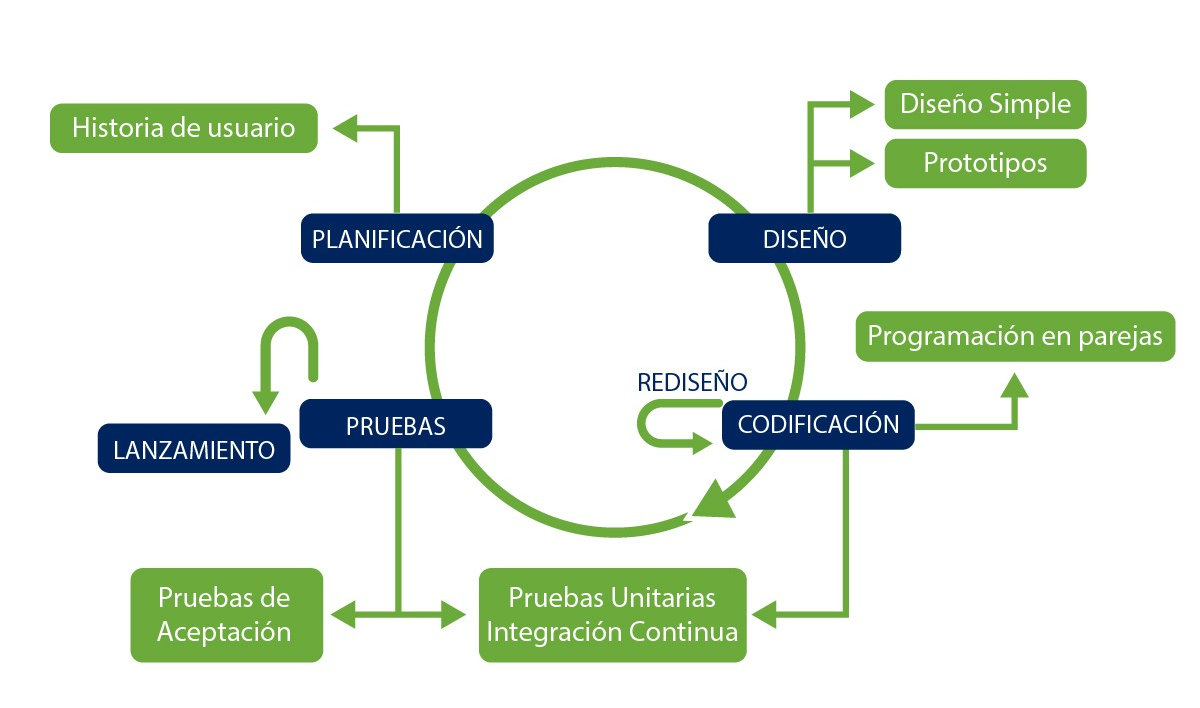
\includegraphics[width=0.7\linewidth]{Images/xp}}
\end{figure}


\section{Herramientas y tecnolog�a de desarrollo de software}

La elecci�n y uso de herramientas y tecnolog�as apropiadas es crucial para el �xito del desarrollo del sistema de gesti�n de citas y servicios de Transconsul \ac{XP}. Al evaluar y seleccionar cuidadosamente estas herramientas, los programadores pueden trabajar de manera m�s eficiente y efectiva, lo que a su vez se traducir� en un producto final de alta calidad. Por lo tanto, es importante llevar a cabo una investigaci�n exhaustiva de las herramientas y tecnolog�as disponibles, con el fin de identificar aquellas que mejor se adapten a las necesidades espec�ficas del proyecto. De esta manera, se puede garantizar que el equipo de desarrollo tenga acceso a las herramientas y tecnolog�as necesarias para trabajar de manera efectiva y lograr los objetivos del proyecto de manera satisfactoria.

\begin{itemize}
	\item Marco de trabajo: Con Django, puedes llevar aplicaciones web desde el concepto hasta el lanzamiento en cuesti�n de horas. Django se encarga de gran parte de las molestias del desarrollo web, por lo que puedes concentrarte en escribir tu aplicaci�n sin necesidad de reinventar la rueda. Es gratuito y de c�digo abierto.
	
	\begin{itemize}
		\item Completamente cargado:
		Django incluye docenas de extras que puedes usar para manejar tareas comunes de desarrollo web. Django se encarga de la autenticaci�n de usuarios, la administraci�n de contenidos, los mapas del sitio, las fuentes RSS y muchas m�s tareas, desde el primer momento.
		\item Tranquilamente seguro:
		Django se toma en serio la seguridad y ayuda a los desarrolladores a evitar muchos errores de seguridad comunes, como la inyecci�n SQL, secuencias de comandos entre sitios, falsificaci�n de solicitudes entre sitios y clickjacking. Su sistema de autenticaci�n de usuarios proporciona una forma segura de administrar cuentas de usuarios y contrase�as.
		\item Extremadamente escalable:
		Algunos de los sitios m�s concurridos del planeta utilizan la capacidad de Django para escalar de forma r�pida y flexible para satisfacer las demandas de tr�fico m�s intensas.
		\item Incre�blemente vers�til:
		Empresas, organizaciones y gobiernos han utilizado Django para construir todo tipo de cosas, desde sistemas de gesti�n de contenidos hasta redes sociales y plataformas inform�ticas cient�ficas.
	\end{itemize}
	
	
	\item Entorno de desarrollo: Visual Studio Code es un editor de c�digo fuente liviano pero potente que se ejecuta en su escritorio y est� disponible para Windows, macOS y Linux. Viene con soporte integrado para JavaScript, TypeScript y Node.js y tiene un rico ecosistema de extensiones para otros lenguajes y tiempos de ejecuci�n (como C++, Java, Python, PHP, Go, .NET)   \\
	Un 'entorno' en Python es el contexto en el que se ejecuta un programa Python que consta de un int�rprete y cualquier cantidad de paquetes instalados. \\
	
	El venv m�dulo admite la creaci�n de "entornos virtuales" livianos, cada uno con su propio conjunto independiente de paquetes Python instalados en sus sitedirectorios. Un entorno virtual se crea sobre una instalaci�n de Python existente, conocida como Python ?base? del entorno virtual, y opcionalmente puede aislarse de los paquetes en el entorno base, de modo que solo est�n disponibles aquellos instalados expl�citamente en el entorno virtual. \\
	
	Cuando se utilizan desde un entorno virtual, las herramientas de instalaci�n comunes, como pip , instalar�n paquetes de Python en un entorno virtual sin necesidad de que se le indique expl�citamente que lo haga.
	
	\item Sistema Gestor de Base de Datos: se utiliz� MySQL, este es un sistema de gesti�n de bases de datos
	relacional, licenciado bajo la GPL de la GNU. Su dise�o multihilo le permite soportar una gran carga
	de forma muy eficiente. Es uno de los gestores m�s usado en el mundo del software libre, debido a
	su gran rapidez y facilidad de uso. Esta gran aceptaci�n, es debida a que existen infinidad de librer�as
	y otras herramientas que permiten su uso a trav�s de gran cantidad de lenguajes de programaci�n,
	adem�s de su f�cil instalaci�n y configuraci�n \citep{daniel_pecos_martinez_postgresql_2024}. Las caracter�sticas fundamentales que
	refleja para su elecci�n por encima de otros gestores de base de datos son: el coste gratuito, la velocidad
	operacional, facilidad de uso y de integraci�n con la mayor parte de los entornos de programaci�n, la
	existencia de una nutrida y activa comunidad \citep{gilfillan_biblia_2003}.
\end{itemize}



Escribir aqu� el cap�tulo 1. Ejemplo de acr�nimo es la \ac{UCI}. Esto es una cita de ejemplo \citep{Ou2013}. En la pr�xima oraci�n se muestra un ejemplo de un acr�nimo en ingl�s. Los sistemas de \ac{SCADA} son de gran importancia para la industria. 

\section{Secci�n de prueba de la \glsentrytext{UCI}} % example on how tu use glossaries or acronym in sections or another moving argument


Esto es una utilizaci�n de una palabra del glosario. El t�rmino \gls{Engine} es utilizado en \ul{este} ejemplo. Esta es una prueba de n�mero: $5.3$ donde se utiliza la coma autom�ticamente como separador.

Esto es una cita de ejemplo \citep{Alfadhlani2011,Mathew2010}.

\begin{figure}[!htb]
\centering
\captionbox{Vista del Arco de Moncloa\label{fig:DSC00461}}
{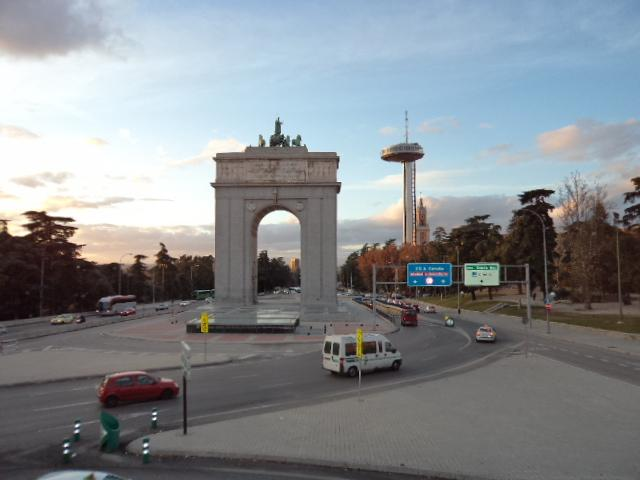
\includegraphics[width=0.7\linewidth]{Images/DSC00461}}
\end{figure}

En la Tabla \ref{Prueba} se observa \dots\\

\begin{table}[!h]
\centering
\captionbox{Caption de Prueba\label{Prueba}}
{
	\begin{tabular}{lllll}
	\hline \textbf{No. 1} & \textbf{No. 2} & \textbf{No. 3} & \textbf{No. 4} & \textbf{No. 5}\\ \hline
	12 & 12 & 56 & 56 &  56 \\ 
	12 & 12 & 56 & 56 &  56 \\
	\hline 
	\end{tabular}
}
\end{table}


\begin{itemize}
\item Uno
\item Dos
\item Tres
\item Cuatro
\item Cinco
\end{itemize}


   \chapter{Caracter�sticas y dise�o del sistema}
\label{chap:chapter2}

\section{Introducci�n al cap�tulo}

En este cap�tulo se desarrolla la propuesta de soluci�n tecnol�gica para enfrentar los problemas de gesti�n de servicios detectados en Transconsul \ac{S.A.}. A partir del an�lisis realizado en el cap�tulo anterior, se describe detalladamente el proceso de dise�o del sistema, desde la definici�n de los m�dulos funcionales hasta la planificaci�n de las entregas y las iteraciones de desarrollo. \\

La soluci�n propuesta se fundamenta en la implementaci�n de un sistema modular que permite gestionar de manera eficiente las citas y servicios ofrecidos por la empresa. En primer lugar, se identifican los roles clave que interactuar�n con el sistema, desde administradores hasta usuarios finales, asegurando que cada actor del proceso cuente con las herramientas necesarias para realizar sus funciones de manera efectiva. Seguidamente, se introducen las Historias de Usuario (HU), que definen de manera clara los requisitos del sistema y las funcionalidades esperadas, proporcionando una visi�n centrada en el usuario y facilitando la priorizaci�n de las tareas de desarrollo. \\

Adem�s, el cap�tulo abarca la planificaci�n de las iteraciones, siguiendo los principios de la metodolog�a �gil Extreme Programming (XP). Esto permite que el desarrollo del sistema sea flexible y adaptable a cambios en los requisitos o retroalimentaci�n del cliente, garantizando la entrega de valor de manera continua. Se presenta un plan de iteraciones detallado que incluye la duraci�n de cada fase, las HU asignadas y el esfuerzo estimado para cada tarea.\\

Finalmente, se aborda el dise�o t�cnico del sistema, que incluye tanto la arquitectura general como los patrones de dise�o utilizados. Se emplean patrones GRASP y GoF, los cuales garantizan que el sistema sea escalable, mantenible y eficiente. Este enfoque modular asegura que la soluci�n pueda crecer y adaptarse a las necesidades cambiantes de la empresa sin comprometer su estabilidad o rendimiento.\\

Este cap�tulo ofrece una visi�n integral del dise�o de la soluci�n propuesta, asegurando que cada aspecto del desarrollo est� alineado con los objetivos de Transconsul S.A. y con las mejores pr�cticas en la creaci�n de sistemas de gesti�n de servicios.\\

\section{Propuesta de soluci�n}

Luego de haber analizado las necesidades del sistema y seleccionado las herramientas para la implementaci�n, se definen los m�dulos a desarrollar para dar soluci�n al problema planteado.

\begin{itemize}
	\item Autenticaci�n y Autorizaci�n: Este m�dulo se encargar� de gestionar la autenticaci�n de usuarios, el registro de cuentas y la autorizaci�n de acceso a diferentes partes de la aplicaci�n.
	\item Gesti�n de Citas: Este m�dulo ser� el n�cleo de la aplicaci�n y se encargar� de permitir a los usuarios programar, aceptar y cancelar citas teniendo en cuenta la disponibilidad diaria de las mismas. Deber� incluir notificaciones de citas programadas y recordatorios autom�ticos.
	\item Gesti�n de Clientes: Manejar� toda la informaci�n relacionada con los clientes, incluyendo su perfil, historial de citas y otra informaci�n relevante.
	\item Gesti�n de Rese�as: Permite a los usuarios dejar rese�as sobre su experiencia con el servicio, las cuales podr�n ser visualizadas y gestionadas por el administrador.
	\item Gesti�n de Trabajadores: Permite a los administradores gestionar la informaci�n de los trabajadores y una  rese�a sobre ellos.
	\item Gesti�n de tramites:Permite a los administradores crear, modificar y eliminar tr�mites disponibles para los usuarios.
	\item Comunicaci�n y Notificaciones: Este m�dulo ser� responsable de facilitar la comunicaci�n entre el bufete de abogados y sus clientes, a trav�s de mensajes de correos electr�nicos que informaran el estado de las citas y servicios solicitados.
	\item Administraci�n del Sistema: Este m�dulo ser� utilizado por los administradores del sistema para gestionar usuarios, configurar ajustes de la aplicaci�n, generar informes y realizar tareas de mantenimiento.
	\item An�lisis y Reportes: Este m�dulo se encargar� de recopilar datos sobre el uso de la aplicaci�n, el rendimiento del sistema y la satisfacci�n del cliente, para generar informes y an�lisis que ayuden a mejorar la eficiencia y calidad del servicio.
\end{itemize}

Para el desarrollo de los m�dulos propuestos se siguen los pasos que establece la metodolog�a �gil XP,
donde se respetar� el esquema que explica \citep{escribano2002introduccion}.

\section{Fase I: Planificaci�n}

Es la fase en la que se define el alcance general del proyecto. En esta el cliente define lo que necesita
mediante la redacci�n de HU y establece la prioridad de cada una. Luego, los programadores estiman los
tiempos de desarrollo en base a esta informaci�n. Las estimaciones realizadas en esta fase son primarias,
debido a que estar�n basadas en datos de muy alto nivel y podr�an variar cuando se analicen en cada ite-
raci�n. Adem�s se toman acuerdos sobre el contenido de la primera entrega y se determina un cronograma
en conjunto con el cliente. Una entrega deber�a obtenerse en no m�s de tres meses \citep{escribano2002introduccion,joskowicz2008reglas}.

\subsection{Historias de Usuarios}

Las HU son la t�cnica que utiliza XP para especificar los requisitos de software, estas deben ser programadas en un tiempo entre una y tres semanas. Si la estimaci�n es superior a las tres semanas, debe ser dividida en dos o m�s historias. Si es menos de una semana, se debe combinar con otra HU. Las estimaciones de esfuerzo, asociado a la implementaci�n de las historias, la establecen los programadores, utilizando como medida el punto. Un punto, equivale a una semana ideal de programaci�n (5 d�as laborables). Las historias, generalmente, valen de 1 a 3 puntos. \citep{escribano2002introduccion}. A continuaci�n se describen las HU definidas para llevar a cabo el desarrollo de los m�dulos.


\begin{userstory}[tb:prueba]
	\storyname{Registro de Usuario}
	\storyuser{Cliente}
	\storyiter{1}
	\storypriority{Alta}
	\storyrisk{Medio}
	\storypoints{0.2}
	\storyprogrammer{Alejandro Santana Viamontes}
	\storydescription{
		Como usuario nuevo, quiero poder registrarme en la aplicaci�n proporcionando mi informaci�n personal, como nombre, direcci�n de correo electr�nico y contrase�a, para acceder a las funcionalidades de la aplicaci�n.
		\begin{itemize}
			\item nombre
			\item direcci�n de correo electr�nico
			\item contrase�a
			\item rectificar contrase�a
		\end{itemize}
	}
	\storyobservation{
		\begin{itemize}
			\item La aplicaci�n debe permitir al usuario completar un formulario de registro con campos para nombre, correo electr�nico y contrase�a.
			\item Los campos del formulario deben validar que la informaci�n ingresada sea v�lida y est� en el formato correcto.
			\item Despu�s de enviar el formulario, la aplicaci�n debe crear una cuenta de usuario y almacenarla en la base de datos.
			\item Se debe enviar un correo electr�nico de confirmaci�n al usuario registrado para verificar su direcci�n de correo electr�nico.
			\item El usuario debe poder iniciar sesi�n despu�s de completar el registro exitosamente.
		\end{itemize}
	}
	%\storyinterface{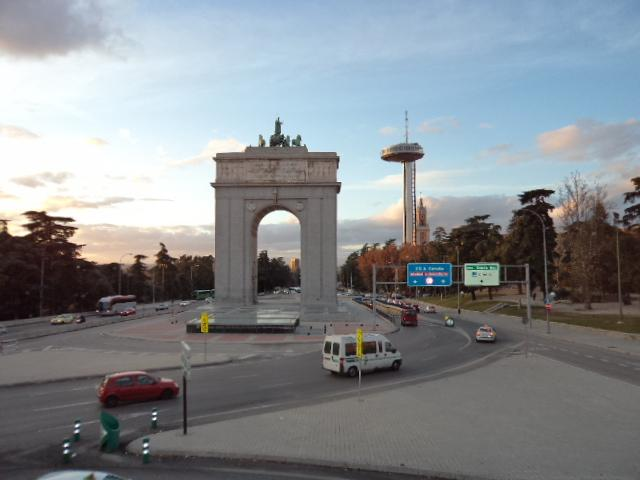
\includegraphics[scale=0.5]{Images/DSC00461}}
\end{userstory}

\begin{userstory}[tb:prueba]
	\storyname{P�gina de Inicio}
	\storyuser{Administrador, Legalizador, Cliente, Notario}
	\storyiter{1}
	\storypriority{Alta}
	\storyrisk{Alto}
	\storypoints{1}
	\storyprogrammer{T�cn. Carlos Brayan R�mila Chorens}
	\storydescription{
		Permite a los usuarios acceder a la pagina de inicio del sistema desde donde se accede a las dem�s funcionalidades del sistema.
	}
	\storyobservation{
	
	}
	%\storyinterface{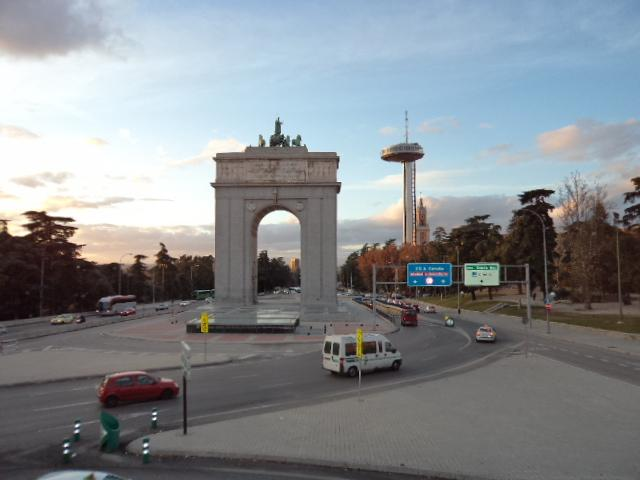
\includegraphics[scale=0.5]{Images/DSC00461}}
\end{userstory}

\begin{userstory}[tb:prueba]
	\storyname{Iniciar Sesi�n}
	\storyuser{Administrador, Legalizador, Cliente, Notario}
	\storyiter{1}
	\storypriority{Alta}
	\storyrisk{Bajo}
	\storypoints{0.2}
	\storyprogrammer{Alejandro Santana Viamontes}
	\storydescription{
		Como usuario registrado, quiero poder iniciar sesi�n en la aplicaci�n utilizando mi direcci�n de correo electr�nico y contrase�a, para acceder a mis datos y realizar acciones dentro de la aplicaci�n.
		\begin{itemize}
			\item direcci�n de correo electr�nico
			\item contrase�a
		\end{itemize}
	}	
	\storyobservation{
		\begin{itemize}
			\item La aplicaci�n debe proporcionar un formulario de inicio de sesi�n con campos para correo electr�nico y contrase�a.
			\item Los campos del formulario deben validar que la informaci�n ingresada sea v�lida y coincida con los datos almacenados en la base de datos.
			\item Despu�s de enviar el formulario, la aplicaci�n debe autenticar al usuario y redirigirlo a la p�gina principal si las credenciales son v�lidas.
			\item Si las credenciales son inv�lidas, la aplicaci�n debe mostrar un mensaje de error al usuario indicando que las credenciales son incorrectas.
			\item La sesi�n del usuario debe mantenerse activa mientras navega por la aplicaci�n, permiti�ndole acceder a las funcionalidades protegidas sin necesidad de volver a iniciar sesi�n.
		\end{itemize}
	}
	%\storyinterface{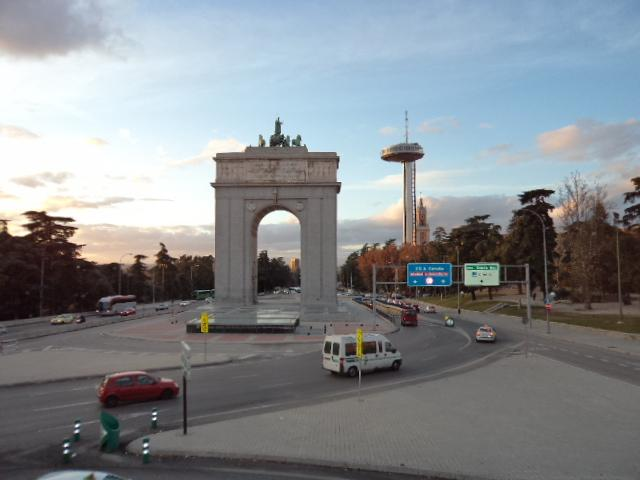
\includegraphics[scale=0.5]{Images/DSC00461}}
\end{userstory}


\begin{userstory}[tb:prueba]
	\storyname{Gesti�n de Perfiles de Usuario}
	\storyuser{Administrador}
	\storyiter{1}
	\storypriority{Media}
	\storyrisk{Bajo}
	\storypoints{0.2}
	\storyprogrammer{T�cn. Carlos Brayan R�mila Chorens}
	\storydescription{
		Como administrador, quiero poder gestionar los perfiles de usuario, incluyendo la capacidad de crear, editar y eliminar cuentas de usuario, para mantener el control sobre qui�n tiene acceso a la aplicaci�n.
		\begin{itemize}
			\item nombre
			\item direcci�n de correo electr�nico
			\item contrase�a
			\item carnet de identidad
			\item rol
		\end{itemize}
	}	
	\storyobservation{
		\begin{itemize}
			\item La aplicaci�n debe proporcionar una interfaz de administraci�n donde el administrador pueda ver una lista de todos los usuarios registrados.
			\item El administrador debe poder crear nuevos perfiles de usuario, proporcionando informaci�n como nombre, direcci�n de correo electr�nico y contrase�a, as� como el rol. 
			\item Se debe implementar la funcionalidad de edici�n para permitir al administrador actualizar la informaci�n de los perfiles de usuario existentes.
			\item El administrador debe poder eliminar cuentas de usuario cuando sea necesario, lo que resultar� en la eliminaci�n permanente de los datos asociados con esa cuenta.
			\item Se deben implementar controles de acceso adecuados para garantizar que solo el administrador tenga acceso a estas funcionalidades de gesti�n de perfiles.
		\end{itemize}
	}
	%\storyinterface{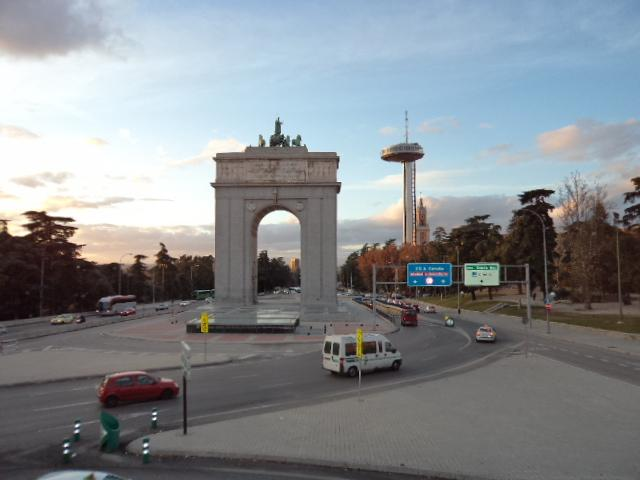
\includegraphics[scale=0.5]{Images/DSC00461}}
\end{userstory}

\begin{userstory}[tb:prueba]
	\storyname{Reservar Cita}
	\storyuser{Cliente}
	\storyiter{1}
	\storypriority{Alta}
	\storyrisk{Alto}
	\storypoints{1}
	\storyprogrammer{T�cn. Carlos Brayan R�mila Chorens}
	\storydescription{
		Permite al usuario acceder a la opci�n de registrar su cita, donde se muestra una p�gina con un formulario a rellenar con los siguientes campos
		\begin{itemize}
			\item Cantidad de Documentos a Legalizar
			\item Obtenci�n de documentos
			\item Fecha
			\item Tr�mite
			\item Con Notario
			\item Motivo
		\end{itemize}
	}	
	\storyobservation{
		\begin{itemize}
		\item El usuario debe estar autenticado en el sistema y con la informaci�n de su perfil completa.
		\item El sistema comprueba que haya disponibilidad para la fecha seleccionada y guarde al reserva en la base de datos.
		\end{itemize}
	}
	%\storyinterface{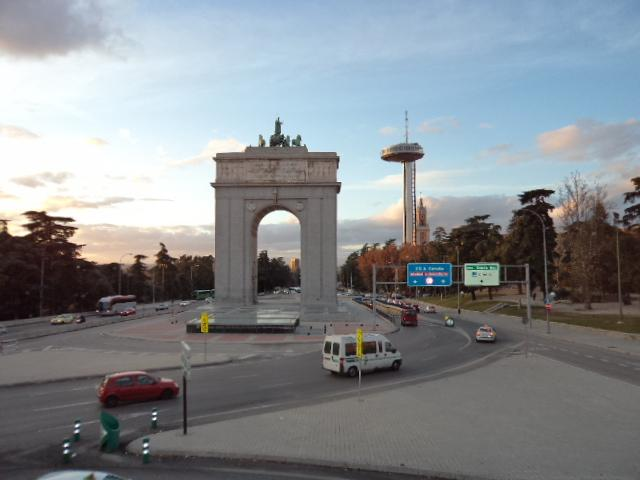
\includegraphics[scale=0.5]{Images/DSC00461}}
\end{userstory}

\begin{userstory}[tb:prueba]
	\storyname{Listar Citas}
	\storyuser{Notario,Legalizador}
	\storyiter{2}
	\storypriority{Alta}
	\storyrisk{Bajo}
	\storypoints{0.3}
	\storyprogrammer{T�cn. Carlos Brayan R�mila Chorens}
	\storydescription{
	Permite a los usuarios listar las citas de todos los clientes donde se muestran la fecha, el cliente, estado y los botones "Aceptar" y "Denegar"
	}
	\storyobservation{
	}	
	%\storyinterface{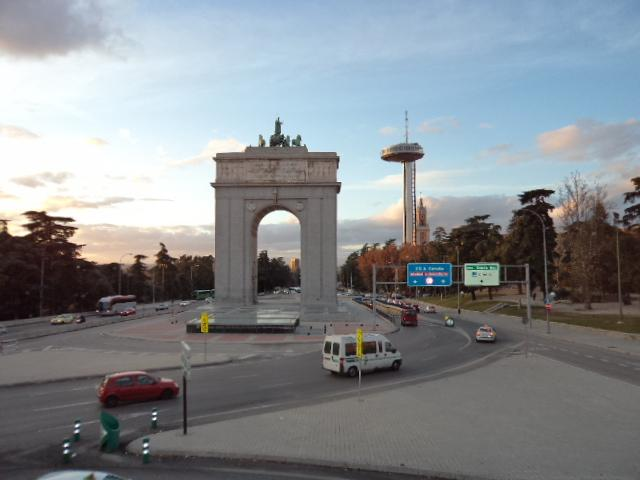
\includegraphics[scale=0.5]{Images/DSC00461}}
\end{userstory}

\begin{userstory}[tb:prueba]
	\storyname{Ver Citas}
	\storyuser{Cliente}
	\storyiter{2}
	\storypriority{Media}
	\storyrisk{Media}
	\storypoints{0.3}
	\storyprogrammer{T�cn. Carlos Brayan R�mila Chorens}
	\storydescription{
		Permite al cliente listar sus citas donde se muestran la fecha y el estado. 
	}
	\storyobservation{
	}	
	%\storyinterface{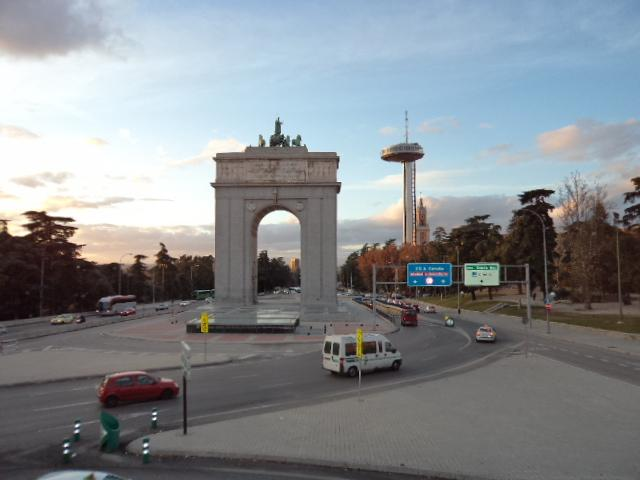
\includegraphics[scale=0.5]{Images/DSC00461}}
\end{userstory}

\begin{userstory}[tb:prueba]
	\storyname{Aceptar Citas}
	\storyuser{Notario,Legalizador}
	\storyiter{2}
	\storypriority{Media}
	\storyrisk{Media}
	\storypoints{0.1}
	\storyprogrammer{T�cn. Carlos Brayan R�mila Chorens}
	\storydescription{
	Permite al usuario cambiar el estado de la cita a "Aceptada" lo que notificar� al cliente a su correo electr�nico.
	}
	\storyobservation{
	}	
	%\storyinterface{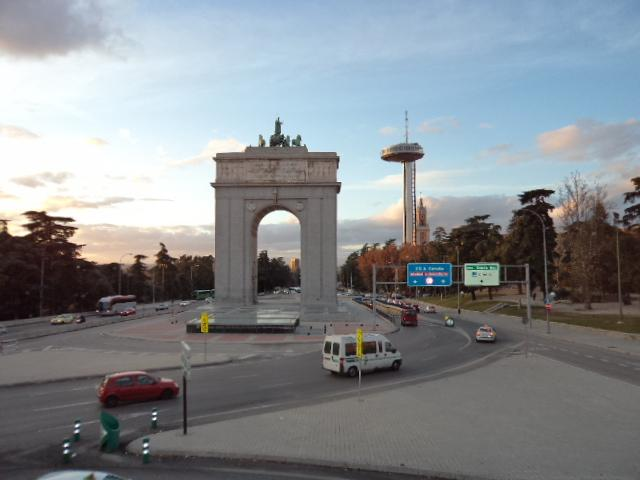
\includegraphics[scale=0.5]{Images/DSC00461}}
\end{userstory}

\begin{userstory}[tb:prueba]
	\storyname{Denegar Citas}
	\storyuser{Notario,Legalizador}
	\storyiter{2}
	\storypriority{Media}
	\storyrisk{Media}
	\storypoints{0.1}
	\storyprogrammer{T�cn. Carlos Brayan R�mila Chorens}
	\storydescription{
		Permite al usuario cambiar el estado de la cita a "Denegada" lo que notificar� al cliente a su correo electr�nico.
	}
	\storyobservation{
	}	
	%\storyinterface{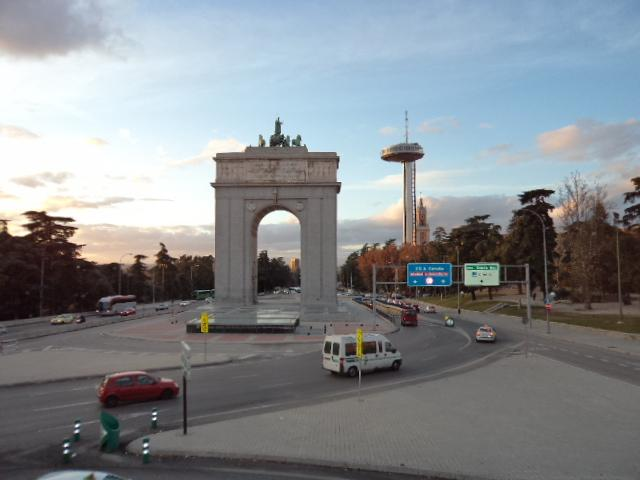
\includegraphics[scale=0.5]{Images/DSC00461}}
\end{userstory}

\begin{userstory}[tb:prueba]
	\storyname{Modificar Perfil Usuario}
	\storyuser{Cliente}
	\storyiter{1}
	\storypriority{Alta}
	\storyrisk{Media}
	\storypoints{0.5}
	\storyprogrammer{T�cn. Carlos Brayan R�mila Chorens, Alejandro Santana Viamontes}
	\storydescription{
		Permite al usuario poder acceder a la opci�n de modificar usuario, donde se muestra una p�gina con un formulario con los datos que el usuario puede modificar los cuales son.
		\begin{itemize}
			\item Nombre
			\item Apellidos
			\item Usuario
			\item Direcci�n
			\item Tel�fono
			\item Carnet de identidad
			\item Foto de perfil
		\end{itemize}
	}	
	\storyobservation{
	}
	%\storyinterface{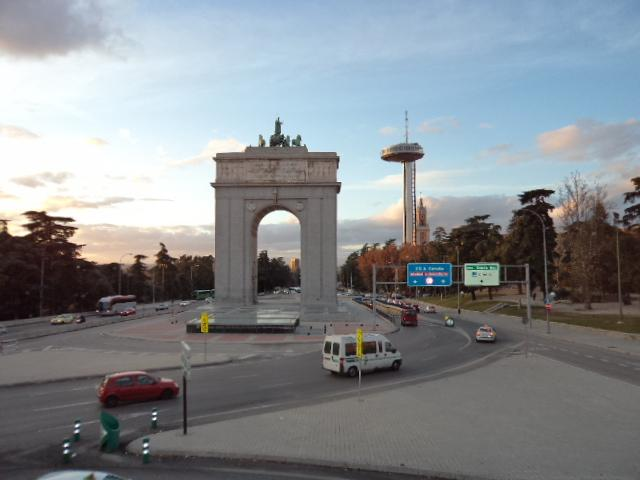
\includegraphics[scale=0.5]{Images/DSC00461}}
\end{userstory}


\begin{userstory}[tb:prueba]
	\storyname{Eliminar Usuario}
	\storyuser{Administrador}
	\storyiter{2}
	\storypriority{Medio}
	\storyrisk{Media}
	\storypoints{0.5}
	\storyprogrammer{T�cn. Carlos Brayan R�mila Chorens}
	\storydescription{
		Permite al usuario poder acceder a la opci�n de eliminar uno o varios usuarios seleccionados, donde se muestra una advertencia con un mensaje de:
	    �Esta seguro?
		No podr� revertir esta acci�n
	}
	\storyobservation{
	}	
	%\storyinterface{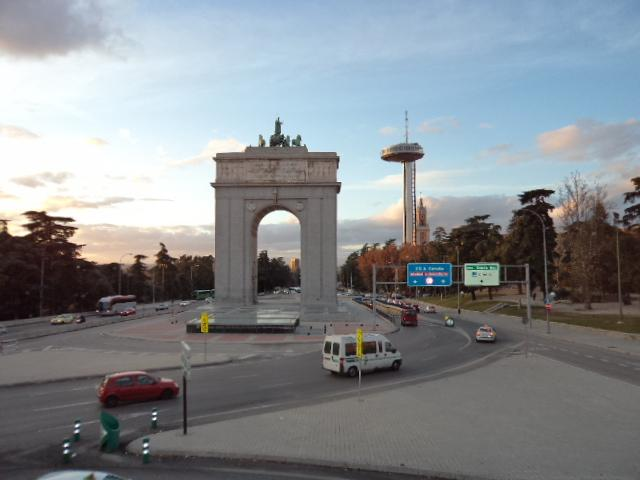
\includegraphics[scale=0.5]{Images/DSC00461}}
\end{userstory}

% Crear Tramite
\begin{userstory}[tb:prueba]
	\storyname{Crear Tramite}
	\storyuser{Administrador}
	\storyiter{2}
	\storypriority{Alta}
	\storyrisk{Media}
	\storypoints{1}
	\storyprogrammer{T�cn. Carlos Brayan R�mila Chorens}
	\storydescription{
		Permite al usuario poder acceder a la opci�n de crear un tr�mite a realizar, donde se muestra una p�gina con un formulario a rellenar con los siguientes datos:
		
		\begin{itemize}
			\item C�digo
			\item Nombre
			\item Descripci�n
			\item Precio
		\end{itemize}
		
		
	}
	\storyobservation{
	}	
	%\storyinterface{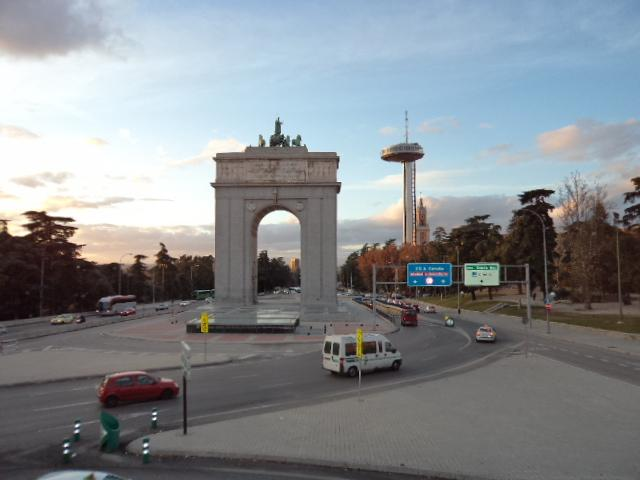
\includegraphics[scale=0.5]{Images/DSC00461}}
\end{userstory}

% Modificar  Tramite
\begin{userstory}[tb:prueba]
	\storyname{Modificar Tramite}
	\storyuser{Administrador}
	\storyiter{2}
	\storypriority{Bajo}
	\storyrisk{Bajo}
	\storypoints{1}
	\storyprogrammer{T�cn. Carlos Brayan R�mila Chorens}
	\storydescription{
		Permite al usuario poder acceder a la opci�n de modificar un tr�mite a realizar, donde se muestra una p�gina con un formulario con los siguientes datos:
		
		\begin{itemize}
			\item C�digo
			\item Nombre
			\item Descripci�n
			\item Precio
		\end{itemize}
		
		
	}	
	\storyobservation{
	}
	%\storyinterface{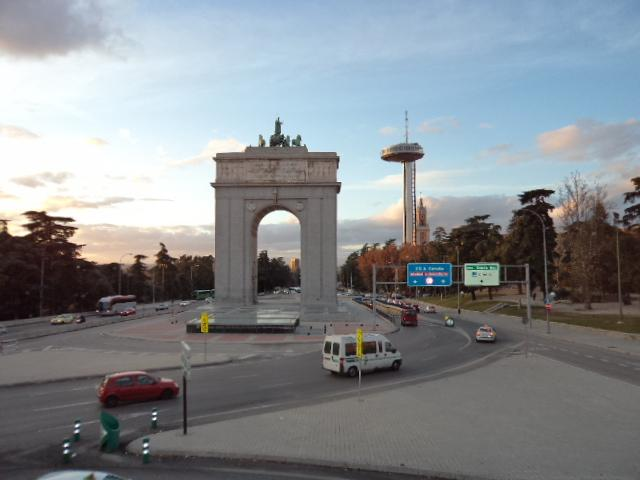
\includegraphics[scale=0.5]{Images/DSC00461}}
\end{userstory}

% Eliminar Tramite
\begin{userstory}[tb:prueba]
	\storyname{Eliminar Tramite}
	\storyuser{Administrador}
	\storyiter{2}
	\storypriority{Media}
	\storyrisk{Medio}
	\storypoints{0.3}
	\storyprogrammer{T�cn. Carlos Brayan R�mila Chorens}
	\storydescription{
		Permite al usuario poder acceder a la opci�n de eliminar tramite o los seleccionados, donde se muestra una advertencia con un mensaje:
		�Esta seguro?
	    No podr� revertir esta acci�n		
		
	}	
	\storyobservation{
	}
	%\storyinterface{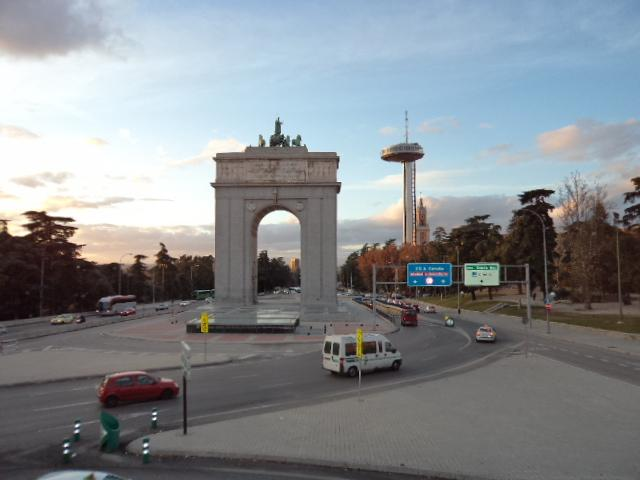
\includegraphics[scale=0.5]{Images/DSC00461}}
\end{userstory}

\begin{userstory}[tb:prueba]
	\storyname{Listar Tramites}
	\storyuser{Administrador}
	\storyiter{2}
	\storypriority{Alta}
	\storyrisk{Bajo}
	\storypoints{0.3}
	\storyprogrammer{T�cn. Carlos Brayan R�mila Chorens}
	\storydescription{
		Permite al usuario listar los tramites, donde se muestra, el c�digo, nombre, descripci�n, precio y los botones de "Agregar", "Modificar" y "Eliminar"		
		
	}	
	\storyobservation{
	}
	%\storyinterface{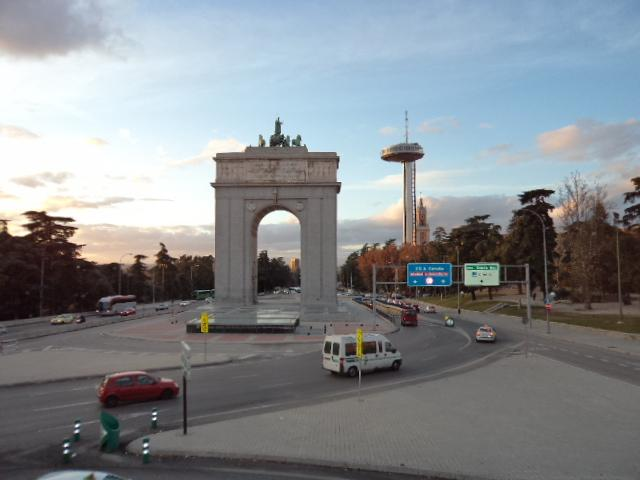
\includegraphics[scale=0.5]{Images/DSC00461}}
\end{userstory}

\begin{userstory}[tb:prueba]
	\storyname{Crear Trabajador}
	\storyuser{Administrador}
	\storyiter{3}
	\storypriority{Baja}
	\storyrisk{Bajo}
	\storypoints{0.2}
	\storyprogrammer{ Alejandro Santana Viamontes
	}
	\storydescription{
		Permite al usuario poder acceder a la opci�n de crear trabajador, donde se muestra una p�gina con un formulario a rellenar con los siguientes datos:
		
		\begin{itemize}
			\item Nombre
			\item Nivel
			\item Descripci�n
			\item Foto
		\end{itemize}
	}
	\storyobservation{
	}	
	%\storyinterface{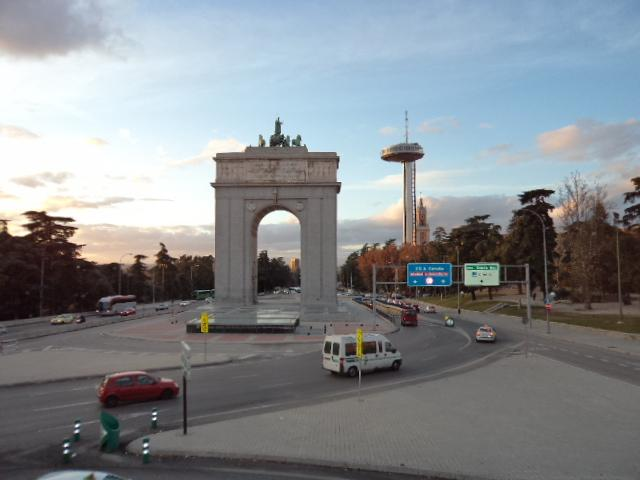
\includegraphics[scale=0.5]{Images/DSC00461}}
\end{userstory}

\begin{userstory}[tb:prueba]
	\storyname{Modificar Trabajador}
	\storyuser{Administrador}
	\storyiter{3}
	\storypriority{Baja}
	\storyrisk{Bajo}
	\storypoints{0.2}
	\storyprogrammer{ Alejandro Santana Viamontes
	}
	\storydescription{
		Permite al usuario poder acceder a la opci�n de modificar trabajador, donde se muestra una p�gina con un formulario a rellenar con los siguientes datos:
		
		\begin{itemize}
			\item Nombre
			\item Nivel
			\item Descripci�n
			\item Foto
		\end{itemize}
	}
	\storyobservation{
	}	
	%\storyinterface{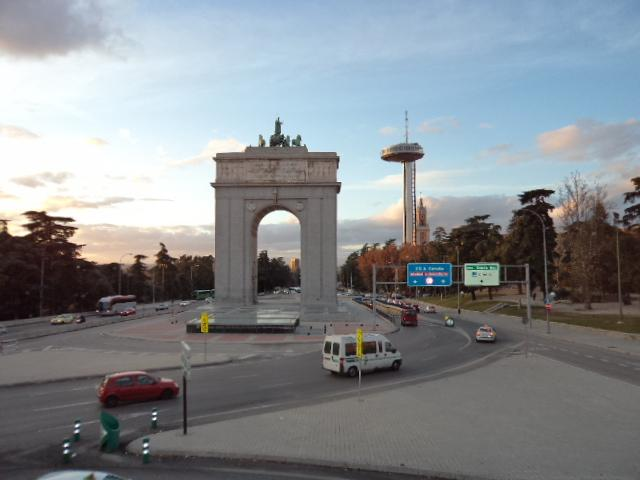
\includegraphics[scale=0.5]{Images/DSC00461}}
\end{userstory}

\begin{userstory}[tb:prueba]
	\storyname{Eliminar Trabajador}
	\storyuser{Administrador}
	\storyiter{3}
	\storypriority{Baja}
	\storyrisk{Bajo}
	\storypoints{0.2}
	\storyprogrammer{ Alejandro Santana Viamontes
	}
	\storydescription{
		Permite al usuario poder acceder a la opci�n de eliminar trabajador, donde se muestra una p�gina con un mensaje de advertencia:
		�Esta seguro?
		No podr� revertir esta acci�n
	}
	\storyobservation{
	}	
	%\storyinterface{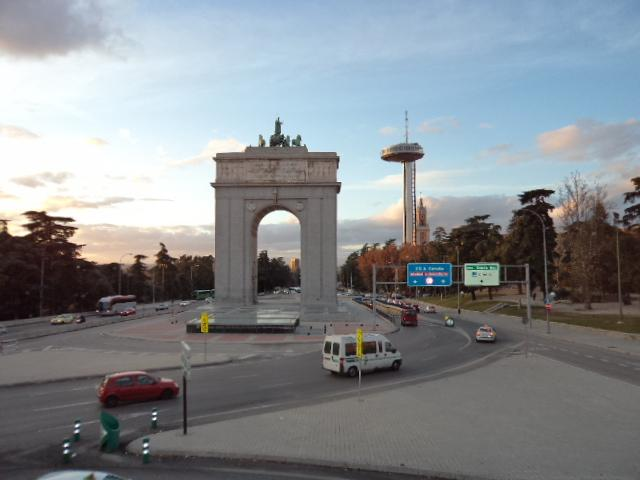
\includegraphics[scale=0.5]{Images/DSC00461}}
\end{userstory}

\begin{userstory}[tb:prueba]
	\storyname{Listar Trabajadores}
	\storyuser{Administrador}
	\storyiter{3}
	\storypriority{Baja}
	\storyrisk{Bajo}
	\storypoints{0.2}
	\storyprogrammer{ Alejandro Santana Viamontes
	}
	\storydescription{
		Permite al usuario listar los trabajadores, donde se muestra el nombre, nivel y descripci�n adem�s de  los botones de "Agregar", "Modificar" y "Eliminar"
	}
	\storyobservation{
	}	
	%\storyinterface{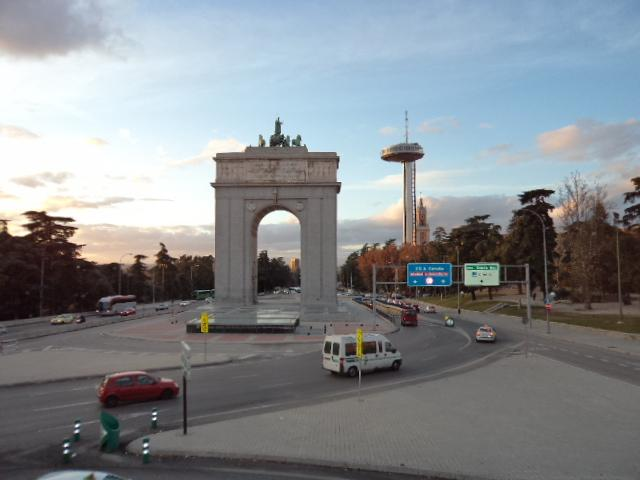
\includegraphics[scale=0.5]{Images/DSC00461}}
\end{userstory}

\begin{userstory}[tb:prueba]
	\storyname{Ver Trabajador}
	\storyuser{Cliente}
	\storyiter{3}
	\storypriority{Media}
	\storyrisk{Bajo}
	\storypoints{0.2}
	\storyprogrammer{ Alejandro Santana Viamontes
	}
	\storydescription{
		Permite al usuario ver la informaci�n de los trabajadores a trav�s de la pagina de inicio.
	}
	\storyobservation{
	}	
	%\storyinterface{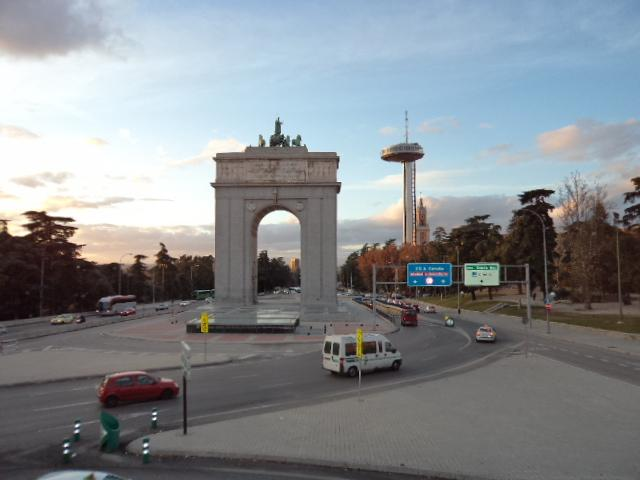
\includegraphics[scale=0.5]{Images/DSC00461}}
\end{userstory}

\begin{userstory}[tb:prueba]
	\storyname{Crear Art�culo}
	\storyuser{Administrador}
	\storyiter{3}
	\storypriority{Baja}
	\storyrisk{Medio}
	\storypoints{0.2}
	\storyprogrammer{T�cn. Carlos Brayan R�mila Chorens}
	\storydescription{
		Permite al usuario poder crear art�culos para el Blog completando un formulario con los siguientes campos.
		\begin{itemize}
		\item T�tulo
		\item Foto
		\item Descripci�n
		\end{itemize}  
	}
	\storyobservation{
	}	
	%\storyinterface{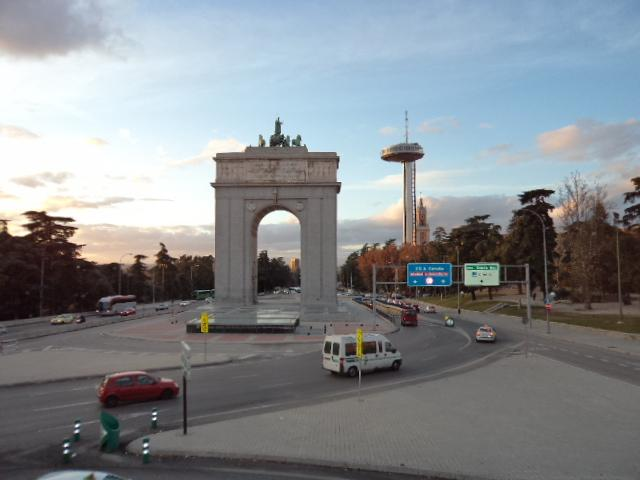
\includegraphics[scale=0.5]{Images/DSC00461}}
\end{userstory}

\begin{userstory}[tb:prueba]
	\storyname{Modificar Art�culo}
	\storyuser{Administrador}
	\storyiter{3}
	\storypriority{Baja}
	\storyrisk{Media}
	\storypoints{0.2}
	\storyprogrammer{T�cn. Carlos Brayan R�mila Chorens}
	\storydescription{
	Permite al usuario poder modificar los art�culos del Blog completando un formulario con los siguientes campos.
	\begin{itemize}
		\item T�tulo
		\item Foto
		\item Descripci�n
	\end{itemize}  
	}
	\storyobservation{
	}	
	%\storyinterface{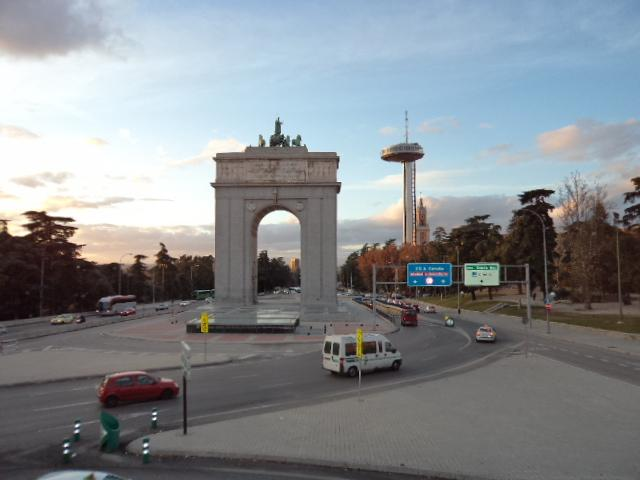
\includegraphics[scale=0.5]{Images/DSC00461}}
\end{userstory}

\begin{userstory}[tb:prueba]
	\storyname{Eliminar Art�culo}
	\storyuser{Administrador}
	\storyiter{3}
	\storypriority{Baja}
	\storyrisk{Media}
	\storypoints{0.2}
	\storyprogrammer{T�cn. Carlos Brayan R�mila Chorens}
	\storydescription{
		Permite al usuario poder acceder a la opci�n de eliminar art�culo, donde se muestra una p�gina con un mensaje de advertencia:
		�Esta seguro?
		No podr� revertir esta acci�n
	}
	\storyobservation{
	}	
	%\storyinterface{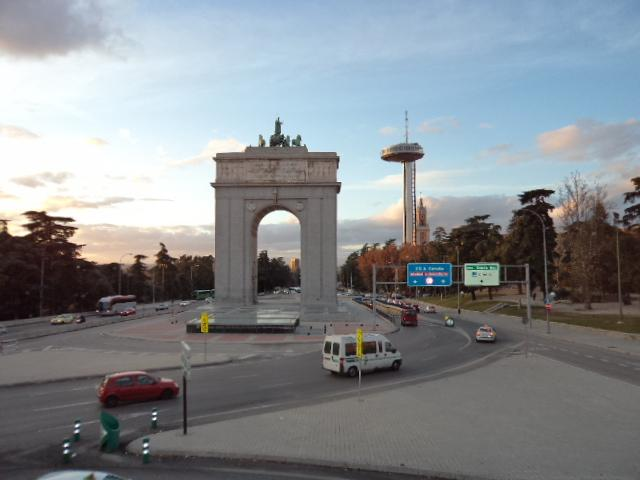
\includegraphics[scale=0.5]{Images/DSC00461}}
\end{userstory}

\begin{userstory}[tb:prueba]
	\storyname{Listar Art�culos}
	\storyuser{Administrador}
	\storyiter{3}
	\storypriority{Alta}
	\storyrisk{Media}
	\storypoints{0.2}
	\storyprogrammer{T�cn. Carlos Brayan R�mila Chorens}
	\storydescription{
		Permite al usuario listar los art�culos, donde se muestra el nombre y la fecha de creaci�n adem�s de los botones de "Crear", "Editar" y "Eliminar"
	}
	\storyobservation{
	}	
	%\storyinterface{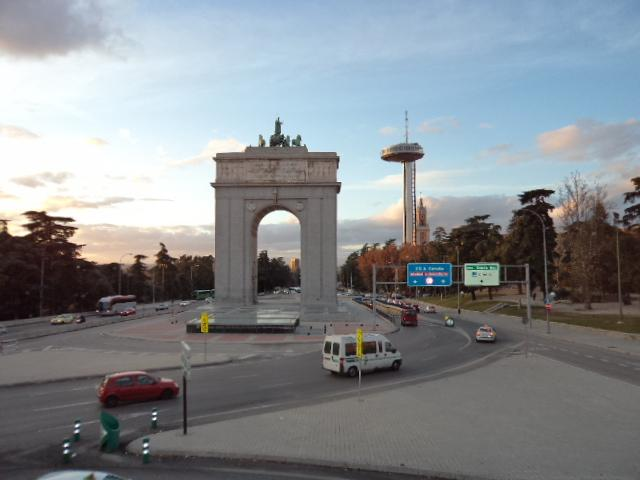
\includegraphics[scale=0.5]{Images/DSC00461}}
\end{userstory}

\begin{userstory}[tb:prueba]
	\storyname{Leer Art�culo}
	\storyuser{Cliente}
	\storyiter{3}
	\storypriority{Baja}
	\storyrisk{Media}
	\storypoints{0.2}
	\storyprogrammer{T�cn. Carlos Brayan R�mila Chorens}
	\storydescription{
		Permite al usuario leer los art�culos del blog.
	}
	\storyobservation{
	}	
	%\storyinterface{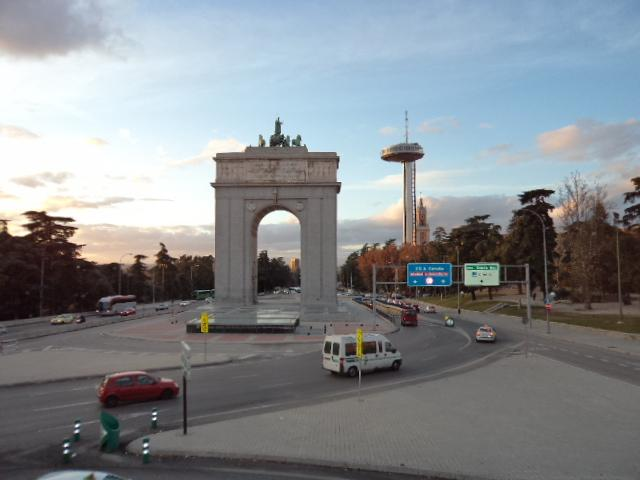
\includegraphics[scale=0.5]{Images/DSC00461}}
\end{userstory}

\begin{userstory}[tb:prueba]
	\storyname{Previsualizar Art�culo}
	\storyuser{Administrador}
	\storyiter{3}
	\storypriority{Alta}
	\storyrisk{Media}
	\storypoints{0.2}
	\storyprogrammer{T�cn. Carlos Brayan R�mila Chorens}
	\storydescription{
		Permite al usuario observar como quedar� el art�culo una vez publicado.
	}
	\storyobservation{
	}	
	%\storyinterface{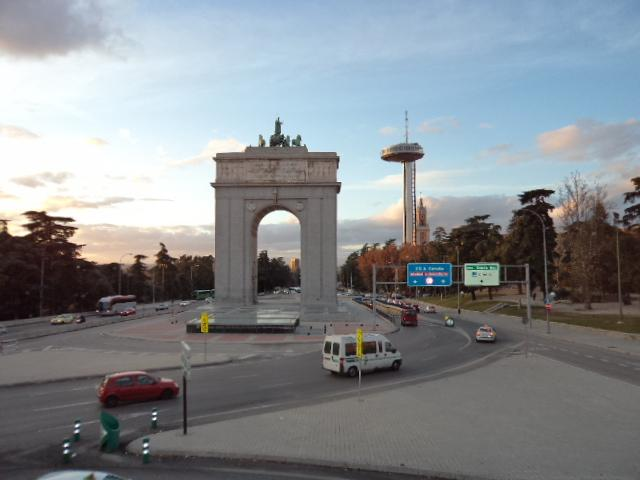
\includegraphics[scale=0.5]{Images/DSC00461}}
\end{userstory}

\begin{userstory}[tb:prueba]
	\storyname{Crear Disponibilidad}
	\storyuser{Notario,Legalizador}
	\storyiter{4}
	\storypriority{Alta}
	\storyrisk{Media}
	\storypoints{0.2}
	\storyprogrammer{T�cn. Carlos Brayan R�mila Chorens}
	\storydescription{
		Permite al usuario crear una disponibilidad completando un formulario con los siguientes campos.
		\begin{itemize}
		\item Fecha 
		\item Cantidad
		\end{itemize}
	}
	\storyobservation{
	}	
	%\storyinterface{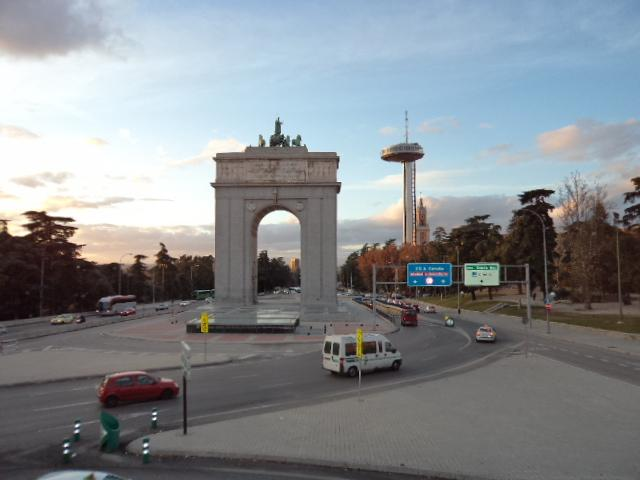
\includegraphics[scale=0.5]{Images/DSC00461}}
\end{userstory}

\begin{userstory}[tb:prueba]
	\storyname{Modificar Disponibilidad}
	\storyuser{Notario,Legalizador}
	\storyiter{4}
	\storypriority{Media}
	\storyrisk{Media}
	\storypoints{0.2}
	\storyprogrammer{T�cn. Carlos Brayan R�mila Chorens}
	\storydescription{
		Permite al usuario modificar una disponibilidad completando un formulario con los siguientes campos.
	\begin{itemize}
		\item Fecha 
		\item Cantidad
	\end{itemize}
	}
	\storyobservation{
	}	
	%\storyinterface{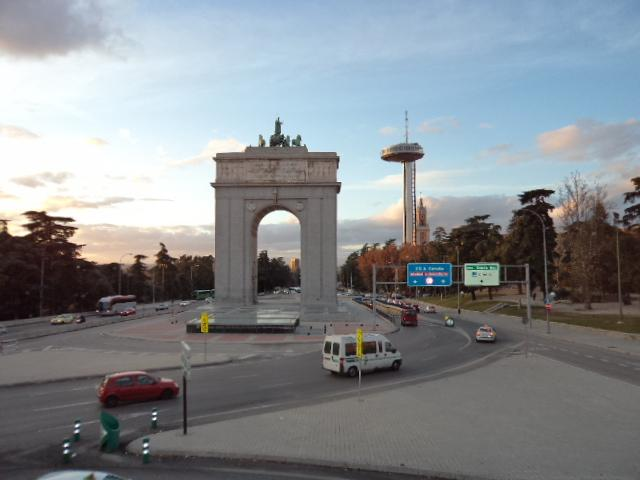
\includegraphics[scale=0.5]{Images/DSC00461}}
\end{userstory}

\begin{userstory}[tb:prueba]
	\storyname{Eliminar Disponibilidad}
	\storyuser{Notario,Legalizador}
	\storyiter{4}
	\storypriority{Alta}
	\storyrisk{Media}
	\storypoints{0.2}
	\storyprogrammer{T�cn. Carlos Brayan R�mila Chorens}
	\storydescription{
		Permite al usuario acceder a la opci�n de eliminar disponibilidad, donde se muestra una p�gina con un mensaje de advertencia:
		�Esta seguro?
		No podr� revertir esta acci�n
	}
	\storyobservation{
	}	
	%\storyinterface{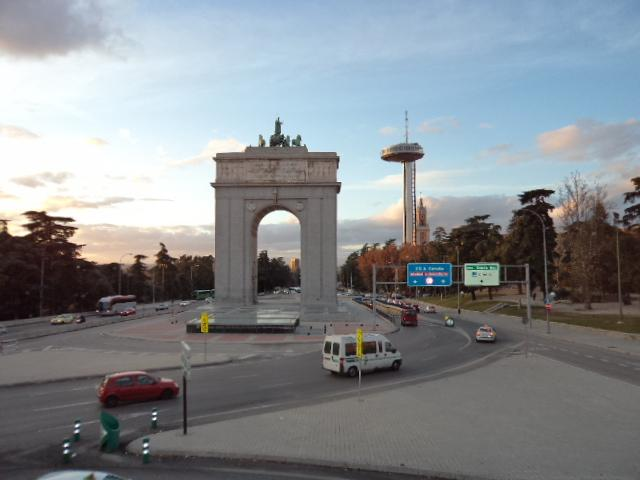
\includegraphics[scale=0.5]{Images/DSC00461}}
\end{userstory}

\begin{userstory}[tb:prueba]
	\storyname{Listar Disponibilidades}
	\storyuser{Notario,Legalizador}
	\storyiter{4}
	\storypriority{Alta}
	\storyrisk{Media}
	\storypoints{0.2}
	\storyprogrammer{T�cn. Carlos Brayan R�mila Chorens}
	\storydescription{
	Permite al usuario listar las disponibilidades, donde se muestra la fecha, cantidad disponibles y cantidad reservadas, adem�s de los botones de "Crear", "Editar" y "Eliminar"
	}
	\storyobservation{
	}	
	%\storyinterface{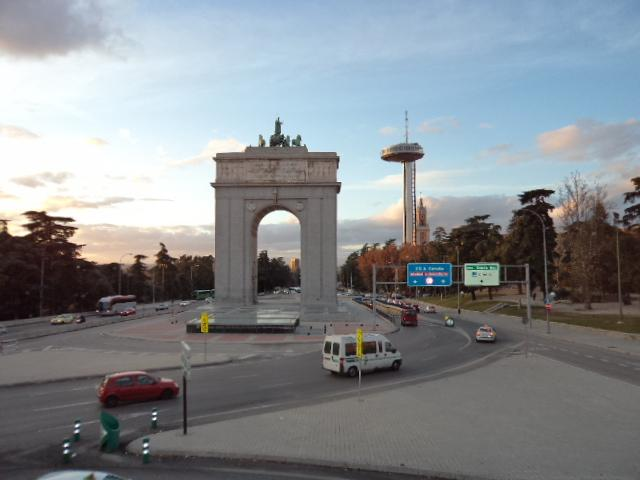
\includegraphics[scale=0.5]{Images/DSC00461}}
\end{userstory}

\begin{userstory}[tb:prueba]
	\storyname{Crear Opini�n}
	\storyuser{Clientes}
	\storyiter{4}
	\storypriority{Alta}
	\storyrisk{Media}
	\storypoints{0.2}
	\storyprogrammer{T�cn. Carlos Brayan R�mila Chorens}
	\storydescription{
		Permite al usuario crear una opini�n sobre los servicios brindados por la empresa.
	}
	\storyobservation{
	}	
	%\storyinterface{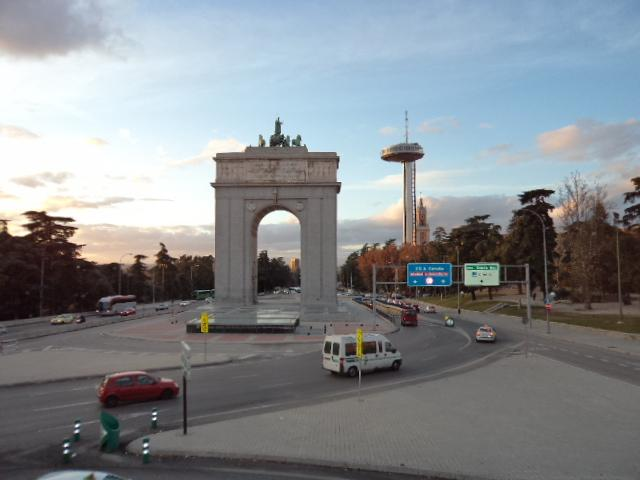
\includegraphics[scale=0.5]{Images/DSC00461}}
\end{userstory}

\begin{userstory}[tb:prueba]
	\storyname{Eliminar Opini�n}
	\storyuser{Administrador}
	\storyiter{4}
	\storypriority{Alta}
	\storyrisk{Media}
	\storypoints{0.2}
	\storyprogrammer{T�cn. Carlos Brayan R�mila Chorens}
	\storydescription{
	Permite al usuario acceder a la opci�n de eliminar opini�n, donde se muestra una p�gina con un mensaje de advertencia:
	�Esta seguro?
	No podr� revertir esta acci�n
	}
	\storyobservation{
	}	
	%\storyinterface{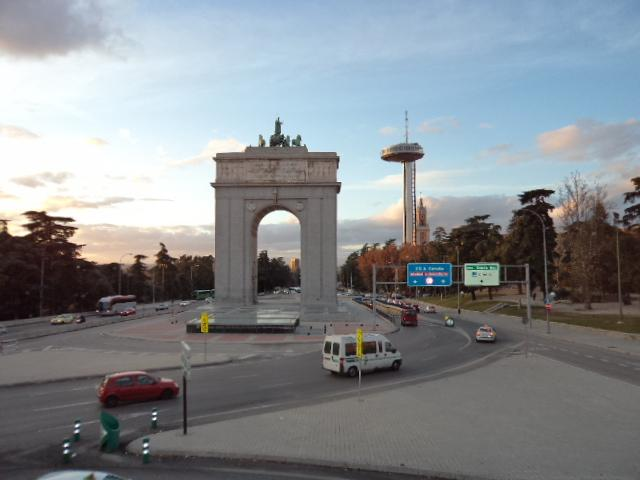
\includegraphics[scale=0.5]{Images/DSC00461}}
\end{userstory}

\begin{userstory}[tb:prueba]
	\storyname{Listar Opiniones}
	\storyuser{Administrador}
	\storyiter{4}
	\storypriority{Alta}
	\storyrisk{Media}
	\storypoints{0.2}
	\storyprogrammer{T�cn. Carlos Brayan R�mila Chorens}
	\storydescription{
		Permite al usuario listar las opiniones hechas por los clientes, donde se muestra la informaci�n de las opiniones as� como el bot�n "Eliminar"
	}
	\storyobservation{
	}	
	%\storyinterface{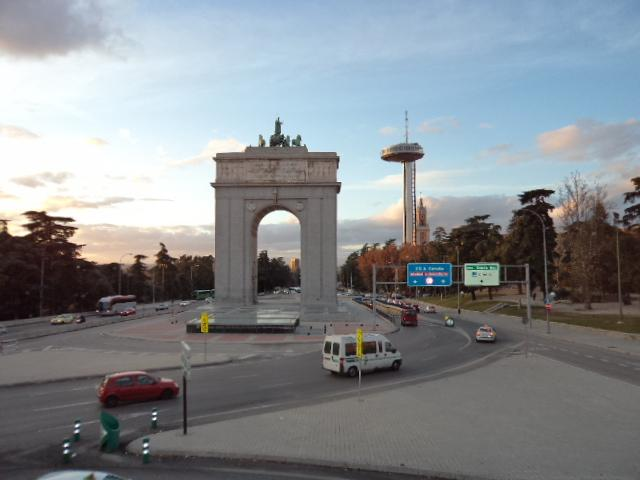
\includegraphics[scale=0.5]{Images/DSC00461}}
\end{userstory}

\begin{userstory}[tb:prueba]
	\storyname{Acceder al blog}
	\storyuser{Cliente}
	\storyiter{4}
	\storypriority{Alta}
	\storyrisk{Media}
	\storypoints{0.2}
	\storyprogrammer{T�cn. Carlos Brayan R�mila Chorens}
	\storydescription{
		Permite al usuario acceder al blog donde podr� ver los art�culos publicados.
	}
	\storyobservation{
	}	
	%\storyinterface{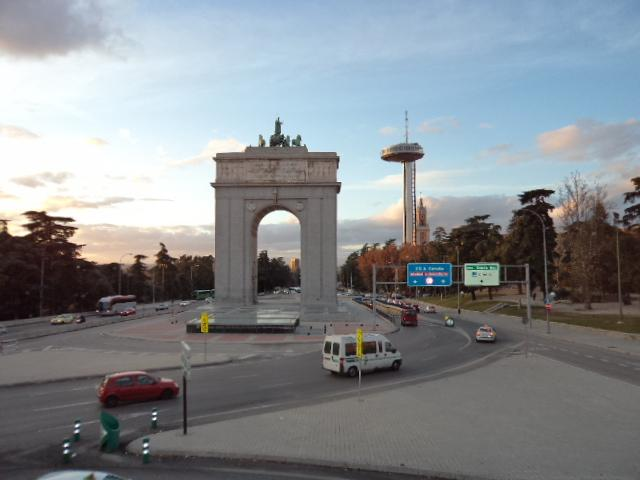
\includegraphics[scale=0.5]{Images/DSC00461}}
\end{userstory}

\begin{userstory}[tb:prueba]
	\storyname{Acceder a Contacto}
	\storyuser{Cliente}
	\storyiter{4}
	\storypriority{Alta}
	\storyrisk{Media}
	\storypoints{0.2}
	\storyprogrammer{T�cn. Carlos Brayan R�mila Chorens}
	\storydescription{
		Permite al usuario acceder a la informaci�n de contacto como direcci�n o tel�fono de la empresa, un mapa con la ubicaci�n y el formulario de soporte.
	}
	\storyobservation{
	}	
	%\storyinterface{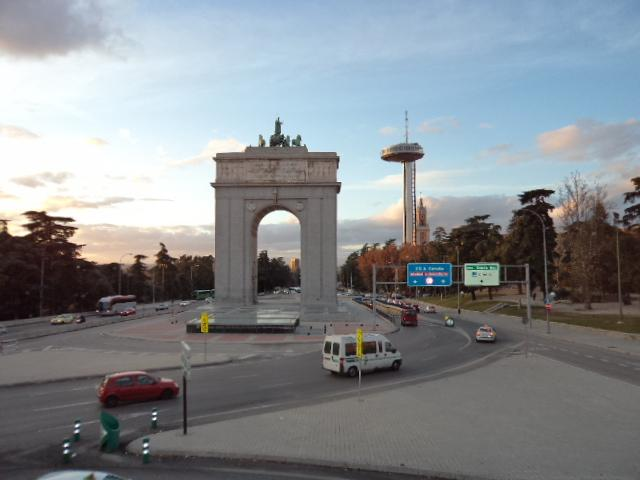
\includegraphics[scale=0.5]{Images/DSC00461}}
\end{userstory}

\begin{userstory}[tb:prueba]
	\storyname{Acceder a Servicios}
	\storyuser{Cliente}
	\storyiter{4}
	\storypriority{Alta}
	\storyrisk{Media}
	\storypoints{0.2}
	\storyprogrammer{T�cn. Carlos Brayan R�mila Chorens}
	\storydescription{
		Permite al usuario acceder a los servicios que brinda la empresa donde se muestran los servicios una breve descripci�n de estos.
	}
	\storyobservation{
	}	
	%\storyinterface{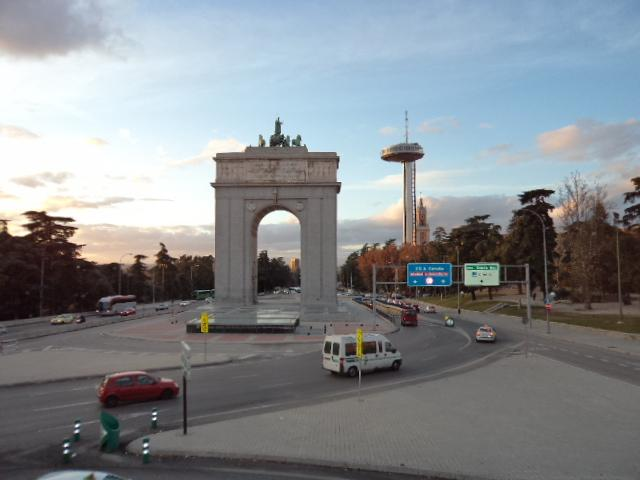
\includegraphics[scale=0.5]{Images/DSC00461}}
\end{userstory}

\begin{userstory}[tb:prueba]
	\storyname{Acceder a Nosotros}
	\storyuser{Cliente}
	\storyiter{4}
	\storypriority{Alta}
	\storyrisk{Media}
	\storypoints{0.2}
	\storyprogrammer{T�cn. Carlos Brayan R�mila Chorens}
	\storydescription{
		Permite al usuario acceder a una rese�a de la empresa donde se muestran datos como los a�os de experiencia, la misi�n y la visi�n de la empresa, entre otros. 
	}
	\storyobservation{
	}	
	%\storyinterface{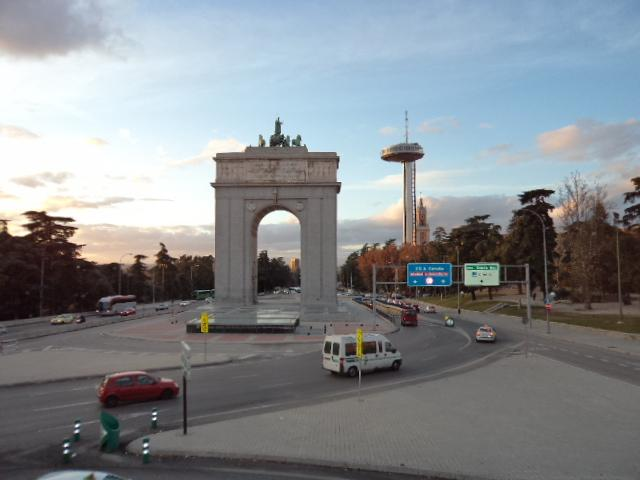
\includegraphics[scale=0.5]{Images/DSC00461}}
\end{userstory}

\subsection{Estimaci�n de esfuerzo por Historia de Usuario}

Se realiza la estimaci�n de esfuerzo que arroja cada HU, con el objetivo de obtener un correcto desarrollo
del sistema. Para una mayor organizaci�n se decide adem�s, asignar a cada iteraci�n el conjunto de historias
agrupadas en correspondencia con el m�dulo al que representen. A continuaci�n se muestra la estimaci�n
realizada:

\subsection{Desarrollo del plan de iteraciones}

Una vez definidas las HU y realizada una previa estimaci�n de esfuerzos, se procede a la planificaci�n de
la etapa de implementaci�n del sistema. En este espacio, se crea el plan de iteraciones, donde se especifica
la prioridad con que se implementar�n las HU organizadas por iteraciones. Teniendo en cuenta el esfuerzo
asociado a las HU y a las prioridades del cliente, se define una versi�n que sea de valor para este.

\begin{effortestimation}
\addentry[1]{ Registro de Usuario}{0.2}
\addentry[1]{ P�gina de Inicio}{1.0}
\addentry[1]{ Iniciar Sesi�n}{0.2}
\addentry[1]{ Gesti�n de Perfiles de Usuario}{0.2}
\addentry[1]{ Reservar Cita}{1.0}
\addentry[1]{ Modificar Perfil Usuario}{0.5}
\addentry[2]{ Listar Citas}{0.3}
\addentry[2]{ Ver Citas}{0.3}
\addentry[2]{ Aceptar Citas}{0.1}
\addentry[2]{ Denegar Citas}{0.1}
\addentry[2]{ Eliminar Usuario}{0.5}
\addentry[2]{ Crear Tramite}{1.0}
\addentry[2]{ Modificar Tramite}{1.0}
\addentry[2]{ Eliminar Tramite}{0.3}
\addentry[2]{ Listar Tramites}{0.3}
\addentry[3]{ Crear Trabajador}{0.2}
\addentry[3]{ Modificar Trabajador}{0.2}
\addentry[3]{ Eliminar Trabajador}{0.2}
\addentry[3]{ Listar Trabajadores}{0.2}
\addentry[3]{ Ver Trabajador}{0.2}
\addentry[3]{ Crear Art�culo}{0.2}
\addentry[3]{ Modificar Art�culo}{0.2}
\addentry[3]{ Eliminar Art�culo}{0.2}
\addentry[3]{ Listar Art�culos}{0.2}
\addentry[3]{ Leer Art�culo}{0.2}
\addentry[3]{ Previsualizar Art�culo}{0.2}
\addentry[4]{ Crear Disponibilidad}{0.2}
\addentry[4]{ Modificar Disponibilidad}{0.2}
\addentry[4]{ Eliminar Disponibilidad}{0.2}
\addentry[4]{ Listar Disponibilidades}{0.2}
\addentry[4]{ Crear Opini�n}{0.2}
\addentry[4]{ Eliminar Opini�n}{0.2}
\addentry[4]{ Listar Opiniones}{0.2}
\addentry[4]{ Acceder al blog}{0.2}
\addentry[4]{ Acceder a Contacto}{0.2}
\addentry[4]{ Acceder a Servicios}{0.2}
\addentry[4]{ Acceder a Nosotros}{0.2}
\end{effortestimation}


\subsection{Plan de duraci�n de las iteraciones}

A continuaci�n, se presenta el plan de duraci�n de las iteraciones. Este plan, tiene como finalidad, mostrar
la duraci�n de cada iteraci�n, as� como el orden en que ser�n implementadas las HU en cada iteraci�n como
se muestra en la tabla siguiente:

\geniterationplan

\subsection{Plan de entregas}

En el plan de entrega que se plantea a continuaci�n, se hace una propuesta de las versiones (releases) del sistema. Cada versi�n se conformar� al finalizar una iteraci�n.

\begin{longtable}[c]{|l|p{3.0cm}|p{3.0cm}|p{3.0cm}|p{3.0cm}|}
	\captionsetup{margin=1.15\leftmargin}
	\caption{Plan de entrega de versiones}
	\label{grid_example_2_rows_5_columns} \\[2ex]
	
	\hline \multicolumn{1}{|c|}{\colorentry{\textbf{Entregable }}} & \multicolumn{1}{c|}{\colorentry{\textbf{ Iteraci�n 1}}} & \multicolumn{1}{c|}{\colorentry{\textbf{ Iteraci�n 2}}} & \multicolumn{1}{c|}{\colorentry{\textbf{ Iteraci�n 3}}} & \multicolumn{1}{c|}{\colorentry{\textbf{ Iteraci�n 4}}} \\ \hline 
	\endfirsthead
	
	\caption{Continuaci�n de la p�gina anterior} \\ 
	\hline \multicolumn{1}{|c|}{\colorentry{\textbf{Columna 1}}} & \multicolumn{1}{c|}{\colorentry{\textbf{Columna 2}}} & \multicolumn{1}{c|}{\colorentry{\textbf{Columna 3}}} & \multicolumn{1}{c|}{\colorentry{\textbf{Columna 4}}} & \multicolumn{1}{c|}{\colorentry{\textbf{Columna 5}}} \\ \hline 
	\endhead
	
	\hline \multicolumn{5}{|r|}{{Contin�a en la siguiente p�gina}} \\ \hline
	\endfoot
	
	\hline
	\endlastfoot
	
	M�dulos & Versi�n 0.1 & Versi�n 0.2 & Versi�n 0.3 &Versi�n 0.4  \\ \hline
	Fecha & 20/9/2024 & 20/10/2024 & 5/11/2024 & 20/11/2024 \\ \hline
	
\end{longtable}


\section{Fase II: Dise�o del sistema}

La plataforma se implement� siguiendo los principios del patr�n arquitect�nico MVT
La arquitectura Modelo-Vista-Template (MVT) es un patr�n de arquitectura de software utilizado por Django. Es una variante del patr�n Modelo-Vista-Controlador (MVC) y se caracteriza por tratar de desacoplar lo m�ximo posible la interfaz de usuario de la l�gica de la aplicaci�n \citep{Sarmiento2019}.
El patr�n MVT se divide en tres componentes principales:

\begin{itemize}
	\item Modelo: El modelo es responsable de manejar los datos y la l�gica de negocio de la aplicaci�n. En otras palabras, el modelo es el encargado de interactuar con la base de datos y proporcionar los datos necesarios a la vista.
	\item Vista: La vista es responsable de presentar los datos al usuario final. En otras palabras, la vista es el encargado de manejar las interfaces gr�ficas y proporcionar informaci�n din�mica al usuario \citep{rafaelD2021}.
	\item 	Plantilla: La plantilla es responsable de definir c�mo se presentan los datos en la vista. En otras palabras, el template define c�mo se estructura y se muestra la informaci�n en la GUI \citep{Sarmiento2019}.
\end{itemize}

El patr�n MVT es una arquitectura de dise�o que se utiliza para crear aplicaciones web eficientes y escalables. La separaci�n de responsabilidades en los componentes del patr�n permite que cada uno cumpla una funci�n clara y definida, lo que facilita su mantenimiento y escalabilidad en el futuro. La reutilizaci�n de c�digo, ya que, al separar las diferentes responsabilidades en componentes individuales, el c�digo se puede escribir una vez y reutilizar en diferentes partes de la aplicaci�n. Esto reduce el tiempo y el costo del desarrollo, y hace que el proceso de programaci�n sea m�s eficiente.


\section{Patrones de dise�o}


Los patrones de dise�o, tratan los problemas que se repiten y que se presentan en situaciones particulares
del dise�o, con el fin de proponer soluciones a ellas. Se encargan de identificar clases, instancias, roles,
colaboraciones entres estas, as� como la distribuci�n de responsabilidades. En resumen,
es una descripci�n de clases y objetos comunic�ndose entre s�, adaptada para resolver un problema de dise�o
general en un contexto particular.

\subsection{Patrones \ac{GRASP}}

\ac{GRASP} son un conjunto de patrones de dise�o de software orientado a objetos que se enfocan en asignar responsabilidades de manera adecuada a las clases y objetos en un sistema. Los patrones de dise�o \ac{GRASP} proporcionan un enfoque pr�ctico para el dise�o orientado a objetos y se pueden aplicar a diferentes etapas del ciclo de vida del software, desde la planificaci�n hasta la implementaci�n. Estos patrones de dise�o pueden ayudar a mejorar el modularidad, la reutilizaci�n, la flexibilidad y la mantenibilidad del software, al tiempo que reducen la complejidad y el acoplamiento entre las clases \citep{CodeScouts2022}.

Patrones de dise�o \ac{GRASP}:

\begin{itemize}
	\item Controlador: maneja las solicitudes entrantes y enviar las respuestas correspondientes a los clientes. El controlador en Django se evidencia a trav�s de una vista y en la configuraci�n de las rutas URL, permitiendo una asignaci�n efectiva de responsabilidades en la gesti�n de solicitudes y l�gica de la aplicaci�n. 
	\item Creador: Django utiliza Creator para crear objetos de modelo. ORM de Django se encarga de crear objetos de modelo y mapearlos a la base de datos. La creaci�n de instancias es unas de las actividades m�s comunes en un sistema orientado a objetos. El patr�n se hace evidente en las clases contenidas dentro del archivo View.py, las cuales tienen la responsabilidad de instanciar los objetos creados con cada sistema de configuraci�n b�sica.
	\item Experto: Django utiliza Expert para asignar responsabilidades de manera adecuada a las clases. En Django, las vistas son responsables de manejar las solicitudes entrantes y las plantillas son responsables de generar las respuestas HTML. Este patron se encuentra aplicado en todas las clases del archivo Models.py.
	\item	Alta Cohesi�n: cada elemento del dise�o debe realizar una labor �nica dentro del sistema, no desempe�ada por el resto de los elementos y auto identificable. Este patr�n est� representado en las clases contenidas dentro del archivo View.py, las cuales tienen una �nica responsabilidad que puede ser CreateView, UpdateView o DeleteView \citep{CodeScouts2022}.
	
\end{itemize}

\subsection{Patrones \ac{GoF}}

Los patrones de dise�o \ac{GoF}) son un conjunto de patrones de dise�o de software orientado a objetos. Estos patrones de dise�o se han convertido en un conjunto cl�sico de patrones de dise�o y son ampliamente utilizados en el dise�o y desarrollo de sistemas de software orientados a objetos. Proporcionan soluciones probadas y efectivas para problemas comunes de dise�o de software orientado a objetos. Cada patr�n describe un problema de dise�o espec�fico y proporciona una soluci�n general que se puede aplicar a diferentes situaciones \citep{gamma1994design}.

Patrones de dise�o \ac{GoF}:

\begin{itemize}
	\item Decorador: agrega funcionalidades adicionales a las vistas. Django utiliza este patr�n para la creaci�n de vistas personalizadas y middleware, permitiendo agregar funcionalidad adicional a las vistas o el procesamiento de solicitudes sin modificar su c�digo principal como la autenticaci�n, cach�, compresi�n \citep{Silva2019}.
\end{itemize}


Una vez definidos los patrones de dise�o, se describen las clases utilizadas en la soluci�n. Siguiendo la metodolog�a XP, se analizan las HU y se descomponen en tareas independientes.

\section{Tarjetas \ac{CRC}}

A continuaci�n, las HU son evaluadas para dividirlas en tareas, cada tarea representa una caracter�stica distinta del sistema y se puede dise�ar una prueba de unidad que verifique cada tarea, estas tareas se
representan por medio de las tarjetas \ac{CRC}.


\begin{figure}[!htb]
	\centering
	\captionbox{Prototipo de Tarjeta \ac{CRC}\label{fig:crc}}
	{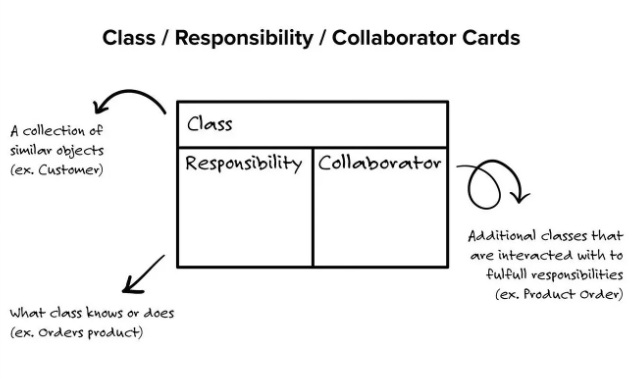
\includegraphics[width=0.7\linewidth]{Images/crc}}
\end{figure}

Como se puede observar en la Figura 2.2, cada tarjeta contiene el nombre de la clase, una descripci�n de
las responsabilidades o m�todos asociados con la clase, as� como la lista de las clases con que se relaciona
o que colaboran con ella. A continuaci�n se describen las tarjetas definidas para la implementaci�n de la
soluci�n.

\begin{crccard}[tb:mytable]
	\crcclass{WorkerView}
	\crcresp{
		\begin{itemize}
			\item worker()
			\item storeWorker()
			\item updateWorker()
			\item deleteWorker()
			\item deleteAllWorker()
			
		\end{itemize}
	}
	\crccolab{
		\begin{itemize}
			\item Worker
			\item User
			\item Middleware
			
		\end{itemize}
	}
\end{crccard}


\begin{crccard}[tb:mytable]
	\crcclass{OpinionView}
	\crcresp{
	\begin{itemize}
		\item opinion()
		\item storeOpinion()
		\item deleteOpinion()
		\item deleteAllOpinion()
		
	\end{itemize}
}
\crccolab{
	\begin{itemize}
		\item Opinion
		\item User
		\item Middleware
		
	\end{itemize}
}
\end{crccard}

\clearpage

\begin{crccard}[tb:mytable]
	\crcclass{UserView}
	\crcresp{
	\begin{itemize}
		\item user()
		\item storeUser()
		\item updateUser()
		\item deleteUser()
		\item deleteAllUser()
		
	\end{itemize}
}
\crccolab{
	\begin{itemize}
		\item User
		\item Middleware
		
	\end{itemize}
}
\end{crccard}

\begin{crccard}[tb:mytable]
	\crcclass{WebView}
	\crcresp{
		\begin{itemize}
			\item home()
			\item service()
			\item about()
			\item testimoniof()
			\item blog()
			\item dashboard()
			
		\end{itemize}
	}
	\crccolab{
		\begin{itemize}
			\item User
			\item Procedure
			\item Opinion
			\item Worker
			\item Middleware
			
		\end{itemize}
	}
\end{crccard}

\begin{crccard}[tb:mytable]
	\crcclass{ProfileView}
	\crcresp{
		\begin{itemize}
			\item profile()
			\item signup()
			\item signin()
			\item signout()
			\item changePassword()
			\item updatePerfil()
			\item updatePhotoPerfil()
			
		\end{itemize}
	}
	\crccolab{
		\begin{itemize}
			\item User
			\item Middleware
			
		\end{itemize}
	}
\end{crccard}

\begin{crccard}[tb:mytable]
	\crcclass{DateView}
	\crcresp{
		\begin{itemize}
			\item reserve()
			\item date()
			\item showDate()
			\item storeDate()
			\item aceptarDate()
			\item cancelarDate()
			
		\end{itemize}
	}
	\crccolab{
		\begin{itemize}
			\item Date
			\item User
			\item Available
			\item Procedure
			\item Middleware
			
		\end{itemize}
	}
\end{crccard}

\begin{crccard}[tb:mytable]
	\crcclass{ProcedureView}
	\crcresp{
		\begin{itemize}
			\item procedure()
			\item storeProcedure()
			\item updateProcedure()
			\item deleteProcedure()
			\item deleteAllProcedure()
		\end{itemize}
	}
	\crccolab{
		\begin{itemize}
			\item Procedure
			\item Middleware
			
		\end{itemize}
	}
\end{crccard}

\begin{crccard}[tb:mytable]
	\crcclass{AvailableView}
	\crcresp{
		\begin{itemize}
			\item available()
			\item storeAvailable()
			\item updateAvailable()
			\item deleteAvailable()
			\item deleteAllAvailable()
		\end{itemize}
	}
	\crccolab{
		\begin{itemize}
			\item Available
			\item Middleware
			
		\end{itemize}
	}
\end{crccard}

\section{Conclusiones del cap�tulo}
	
	En el presente cap�tulo se ha descrito en detalle el dise�o y las caracter�sticas principales del sistema propuesto para Transconsul \ac{S.A.}, con el objetivo de mejorar la gesti�n de sus servicios legales. A trav�s de la implementaci�n de un enfoque modular, una metodolog�a �gil y herramientas de dise�o avanzadas, se ha logrado establecer una soluci�n t�cnica robusta y alineada con los requerimientos de la empresa. A continuaci�n, se destacan las conclusiones principales:
	
	\begin{enumerate}
		\item \textbf{Dise�o modular y flexible:} El sistema propuesto se basa en un dise�o modular que permite una implementaci�n escalonada de las funcionalidades, facilitando tanto el desarrollo como el mantenimiento. Esta estructura asegura que el sistema pueda adaptarse a las necesidades cambiantes de la empresa y escalar conforme se incrementen los servicios ofrecidos o se modifiquen los procesos.
		
		\item \textbf{Historias de Usuario (HU) como gu�a central:} La definici�n clara y detallada de las Historias de Usuario (HU) ha sido fundamental para captar de manera precisa los requerimientos de los diferentes actores del sistema, lo que ha permitido priorizar las funcionalidades cr�ticas y garantizar que el desarrollo est� centrado en las necesidades del cliente final.
		
		\item \textbf{Planificaci�n iterativa con XP:} La metodolog�a �gil \textbf{Extreme Programming (XP)} ha proporcionado un marco de trabajo eficiente, que no solo permite un desarrollo continuo, sino tambi�n una retroalimentaci�n constante con el cliente, asegurando que los cambios puedan incorporarse r�pidamente sin afectar la calidad del producto final. El plan de iteraciones y el plan de entregas garantizan un desarrollo ordenado y progresivo.
		
		\item \textbf{Uso de patrones de dise�o (GRASP y GoF):} La aplicaci�n de patrones de dise�o, como \textbf{GRASP} y \textbf{GoF}, ha contribuido significativamente a una mejor organizaci�n del c�digo y a una asignaci�n m�s eficiente de las responsabilidades entre las clases del sistema. Estos patrones garantizan un dise�o coherente, reutilizable y f�cil de mantener, reduciendo la complejidad a medida que el sistema crece.
	\end{enumerate}
	
	En conclusi�n, este cap�tulo ha establecido las bases t�cnicas y funcionales necesarias para la implementaci�n del sistema, asegurando que la soluci�n propuesta no solo cumpla con los objetivos establecidos, sino que tambi�n sea lo suficientemente flexible y escalable para evolucionar junto con las necesidades de Transconsul \ac{S.A.}.
	


  \chapter{Implementaci�n y prueba del sistema}
\label{chap:chapter3}

\section{Introducci�n al cap�tulo}

En el presente cap�tulo se detallan las iteraciones realizadas durante la etapa de construcci�n de los
m�dulos propuestos, adem�s se exponen las tareas de ingenier�a generadas para cada HU que que fueron
definidas, as� como las pruebas de aceptaci�n planificadas para el sistema. De esta forma es obtenido un
producto funcional probado y listo para entregar al cliente al final de cada iteraci�n como propone XP.

\section{Fase III: Desarrollo}

En esta fase, XP plantea que las HU seleccionadas para ser implementadas se realizan durante el transcurso de la iteraci�n a la que pertenecen. Por estas razones, se lleva a cabo una revisi�n del plan de iteraciones
y se modifican en caso de ser necesario. Como parte de este plan se descomponen las HU en tareas de
ingenier�a \citep{joskowicz2008reglas}.

\section{Tareas de ingenier�a}

Las tareas de ingenier�a pueden estar descritas por un lenguaje t�cnico y no ser necesariamente entendibles por el cliente. Tienen como objetivo definir cada una de las actividades que dan cumplimiento a las
HU, de forma tal que se entienda lo que el sistema tiene que hacer y facilite su construcci�n. Se describen
algunas de las tareas de ingenier�a correspondientes a las HU del sistema, el resto pueden ser consultadas en
los anexos. Para una mayor organizaci�n, se definen en correspondencia con las iteraciones definidas como
se manifiesta a continuaci�n


\subsection{Tareas de ingenier�a para la Iteraci�n I}

\subsection{Tareas de ingenier�a para la Iteraci�n II}

\subsection{Tareas de ingenier�a para la Iteraci�n III}

Con las tareas de ingenier�a definidas, se hace necesario establecer un conjunto de pruebas para comprobar la calidad de la soluci�n implementada. Luego, se analizan estos casos de prueba y se ejecutan, lo que permite medir el nivel de cumplimiento con los objetivos de implementaci�n trazados y el nivel de
satisfacci�n del cliente. As� lo propone XP.

\section{Fase IV: Pruebas}

Las pruebas son un conjunto de actividades que se pueden planificar por adelantado y llevar a cabo sistem�ticamente. Por esta raz�n, se deben definir en el proceso de la ingenier�a del software. Todo esto, contribuye a elevar la calidad de los productos desarrollados y a la seguridad de los programadores a la hora de introducir cambios o modificaciones. \\
La metodolog�a XP divide las pruebas en dos grupos: pruebas unitarias, desarrolladas por los programadores, encargadas de verificar el c�digo de forma autom�tica y las pruebas de aceptaci�n, destinadas a evaluar si al final de una iteraci�n se obtuvo la funcionalidad requerida, adem�s de comprobar que dicha
funcionalidad sea la esperada por el cliente \citep{escribano2002introduccion}. \\
Se decide realizar las pruebas de aceptaci�n a los m�dulos implementados, debido a que el objetivo de estas, es verificar que el sistema cumpla con los requisitos establecidos por el usuario. De esta forma se puede obtener el grado de satisfacci�n del cliente.

\section{Pruebas de aceptaci�n}

Las pruebas de aceptaci�n son especificadas por el cliente, se centran en las caracter�sticas y funcionalidades generales del sistema que son visibles. Estas pruebas derivan de las HU que se han implementado como parte de la liberaci�n del software. Una prueba de aceptaci�n es como una caja negra. Cada una de ellas representa una salida esperada del sistema. Es responsabilidad del cliente verificar la correcci�n y toma de decisiones acerca de estas pruebas. A continuaci�n, se muestra una representaci�n de las pruebas de aceptaci�n a realizarse en cada iteraci�n.

\subsection{Pruebas de aceptaci�n para la Iteraci�n I}

\subsection{Pruebas de aceptaci�n para la Iteraci�n II}

\subsection{Pruebas de aceptaci�n para la Iteraci�n III}

\subsection{An�lisis de las pruebas de aceptaci�n}

\section{Conclusiones del cap�tulo}

En este cap�tulo se especific� el proceso de implementaci�n del sistema a partir del desglose de las HU en tareas de ingenier�a, lo que permiti� especificar los procedimientos necesarios para dar cumplimiento a cada HU. Adem�s se definieron y aplicaron las pruebas de aceptaci�n a las funcionalidades de los m�dulos desarrollados. Estas pruebas permitieron detectar una falla en el sistema y corregirla, lo que posibilit� mejorar la operabilidad del mismo.

  \conclusions

Con el desarrollo de la presente investigaci�n se arriba a la siguiente conclusi�n:

\begin{itemize}
	\item La implementaci�n de los m�dulos propuestos incorpora funcionalidades asociadas con la gesti�n de servicios de Transconsul S.A., permitiendo mejorar la imagen y la efectividad con el p�blico.
\end{itemize}
  \suggestions

A partir de los resultados obtenidos se recomienda:

\begin{itemize}
	\item Desarrollar una aplicaci�n android para facilitar el uso del sistema por parte del cliente
\end{itemize}
  \appendixes

\begin{addendum}
	\chapter{Proyectos y Avales}
    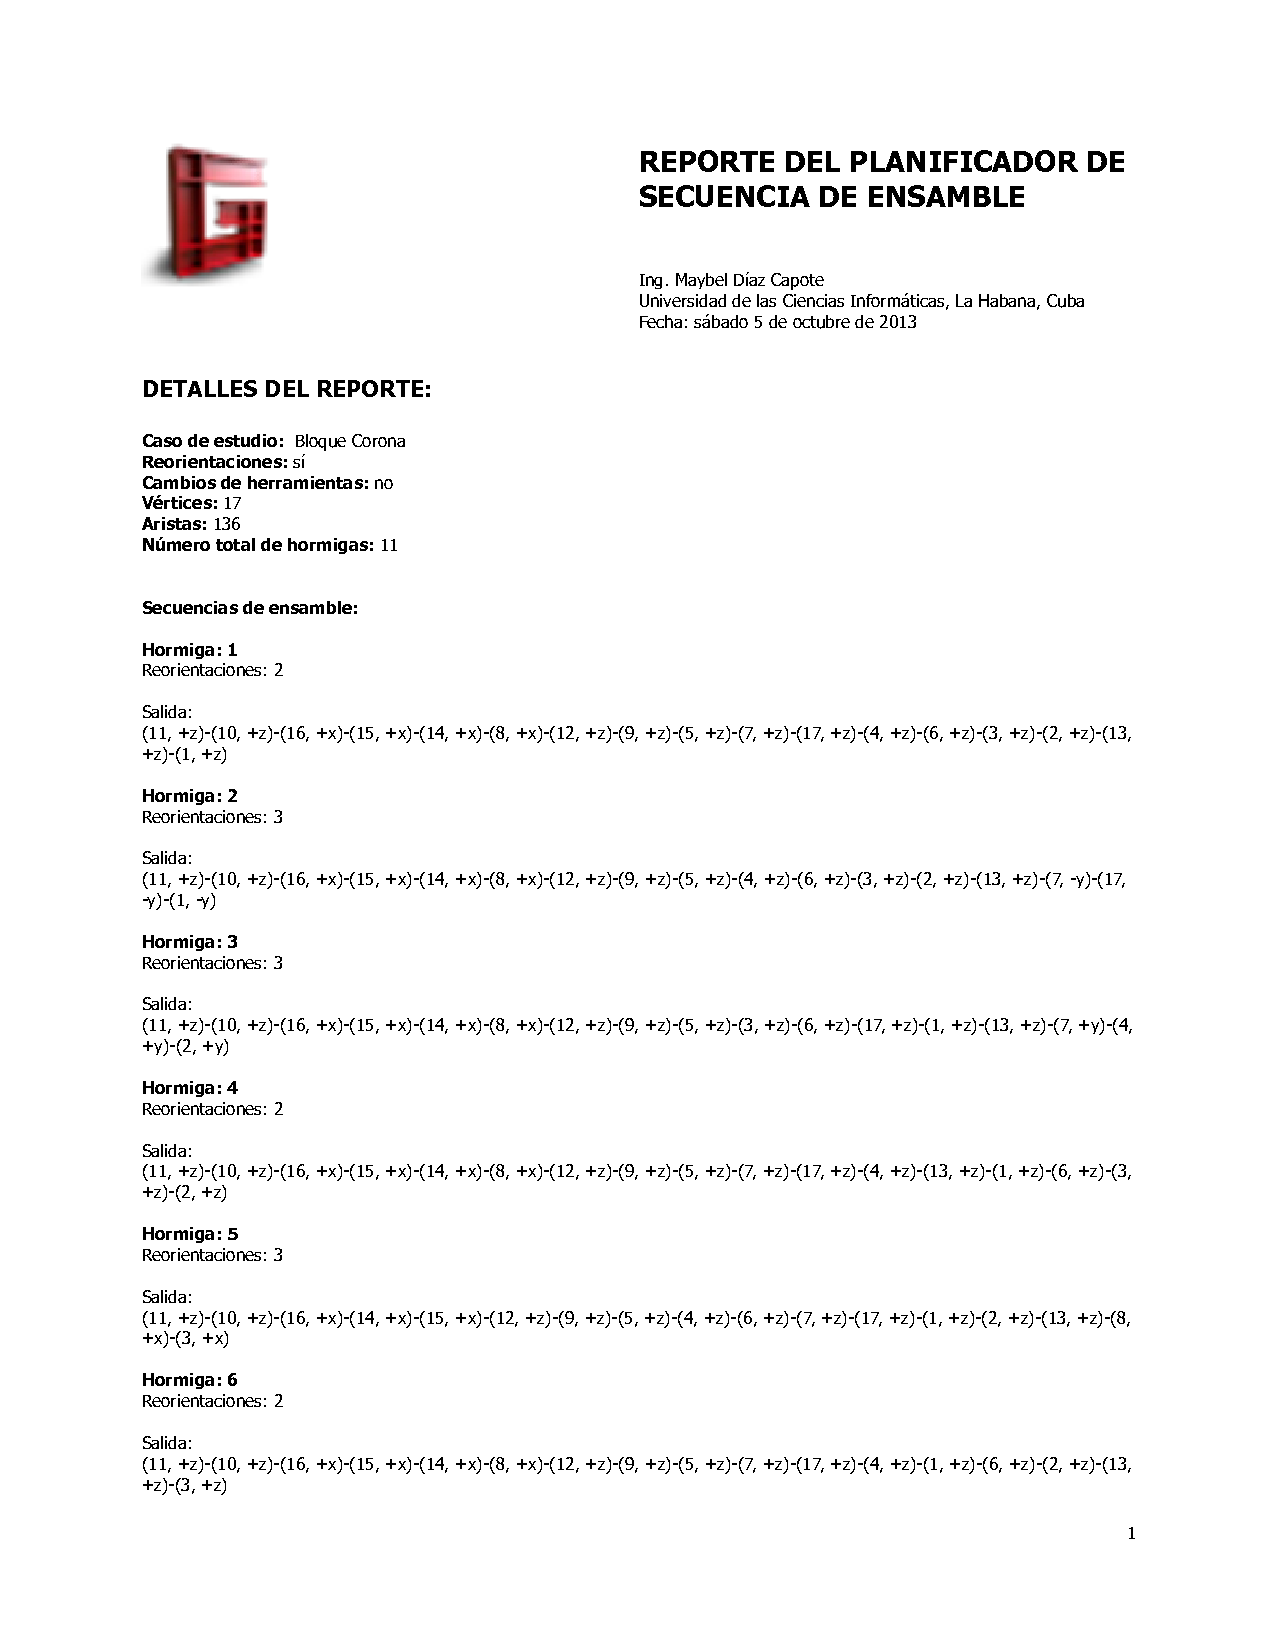
\includegraphics[scale=0.45]{Anexos/BloqueCoronaReport}
   
  	\chapter{Otro reporte}
  	\section{Otra secci�n de muestra}
  	De una sola \hypertarget{word}{sentencia} 
	\section{Otro ensamble Industrial}
	\label{anx:ensambleindustrial}
	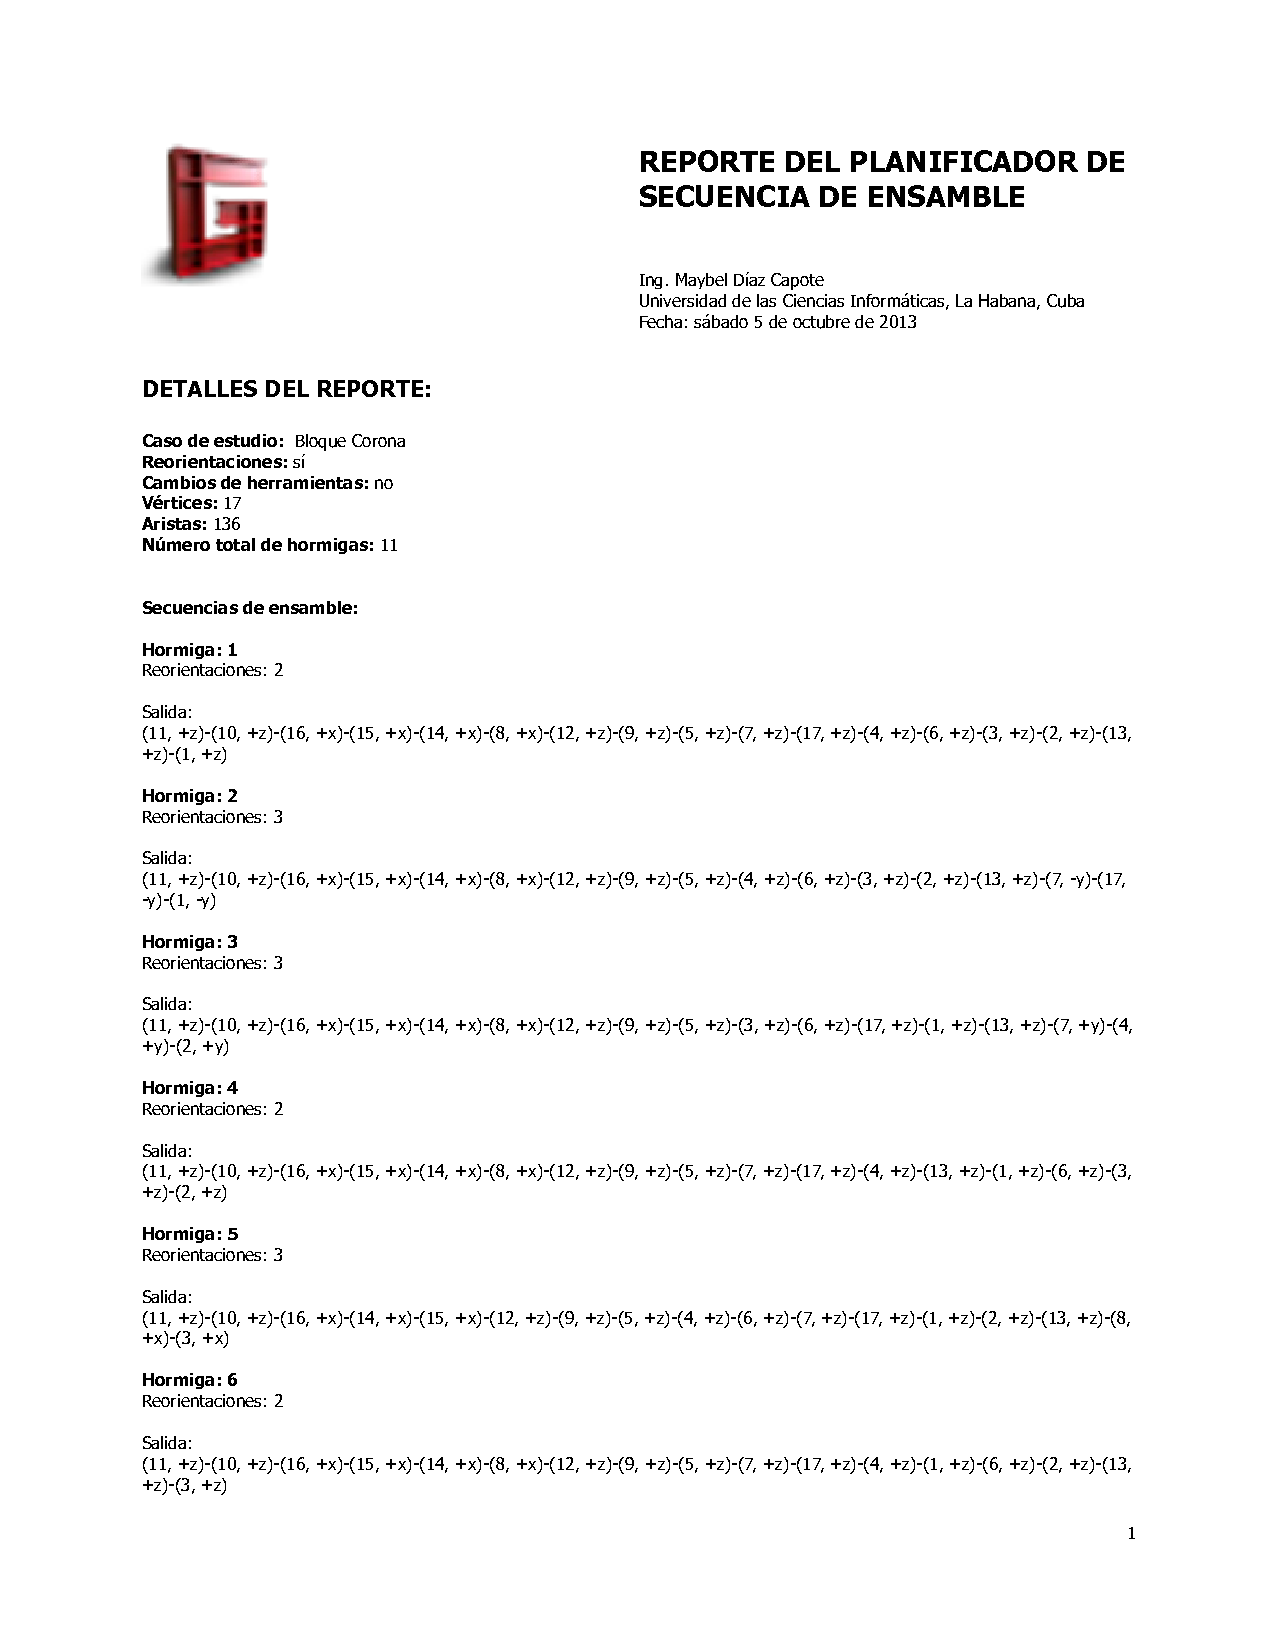
\includegraphics[scale=0.45]{Anexos/BloqueCoronaReport}
\end{addendum}

	\addappendix[bloque]{Anexos/BloqueCoronaReport}
%\addappendix[controlador]{Anexos/ControladorIndustrialReport}

  
  
\end{document}

\end{lstlisting}
